\documentclass{article}
\usepackage[utf8]{inputenc}
\usepackage{graphicx}
\usepackage{hyperref}
\usepackage{listings}
\usepackage{csquotes}
\author{Felix Bello, Gilles Brunner}
\title{Arbeitsauftrag 2}
\begin{document}
	\maketitle
	\section{Einführung}
	Nachstehend wird beschrieben, wie wir für eine Wordpress-Installation im Rahmen des Moduls IKS vorgehen. Da wir die Aufgabe auf unserem Debian-Server statt einem CentOS-Server lösen, gibt es einige Unterschiede bei gewissen Namen: Apache ist nicht unter httpd zu finden, sondern Apache2 und der Benutzer und die Gruppe für unseren Webpfad ist \textit{www-data} (das nur als Info, damit es bei der Aufführung unsere Pfade und 	Benutzerberechtigungen kein Durcheinander gibt.) Mit Ausnahme von Linux (versteht sich von selbst) und PHP, das wir für unsere Wordpress-Installation nicht extra konfigurieren mussten, widmen wir uns nachfolgend den einzelnen Komponenten unseres LAMP-Stacks.
	\section{LAMP}
	Begonnen wird die Aufgabe mit der Instatallation eines LAMP-Stacks. In unserem Fall bezieht sich dieses Akronym auf: Linux, Apache, MariaDB und PHP. Es gibt Scripts für LAMP-Installationen, aber wir haben uns dafür entschieden, die erforderlichen Pakete direkt über den Paketmanager zu beziehen. Da wir unsere Arbeit gemeinsam machen sollten, haben wir uns über SSH mit unserem Server verbunden und mit screen eine Session geteilt, damit beide sich aktiv beteiligen können und immer genau sehen, was der andere macht. Nachfolgend die Terminal-Befehle und entsprechenden Screenshots zur Illustration:
	\linebreak
	SSH-Verbindung:
	\begin{lstlisting}[language=bash]
	$ ssh user@externe-ip-adresse-server
	\end{lstlisting}
	Wechsel zu Root-Rechten (SSH-root login wurde ausgeschaltet)
	\begin{lstlisting}[language=bash]
	$ sudo su
	\end{lstlisting}
	Starten einer screen-session, damit man sich ein Terminal teilen kann:
	\begin{lstlisting}[language=bash]
	# screen -S newScreen
	\end{lstlisting}
	Und entsprechend der zweite User, session joinen:
	\begin{lstlisting}[language=bash]
	# screen -x session-nummer
	\end{lstlisting}
	Installation der für ein LAMP-Stack erforderlichen Pakete:
	\begin{lstlisting}[language=bash]
	# apt-get install mariadb-client-10.0
	  mariadb-server-10.0 apache2 apache2-doc 
	  php5 php5-mysql libapache 2-mod-php5
	\end{lstlisting}
	Nach Ausführung dieses Befehls wird ein ein Konfigurationsfenster zur Einrichtung unserer Datenbank \textit{MariaDB} erscheinen, das wie folgt aussieht:
	\newline
	\newline
	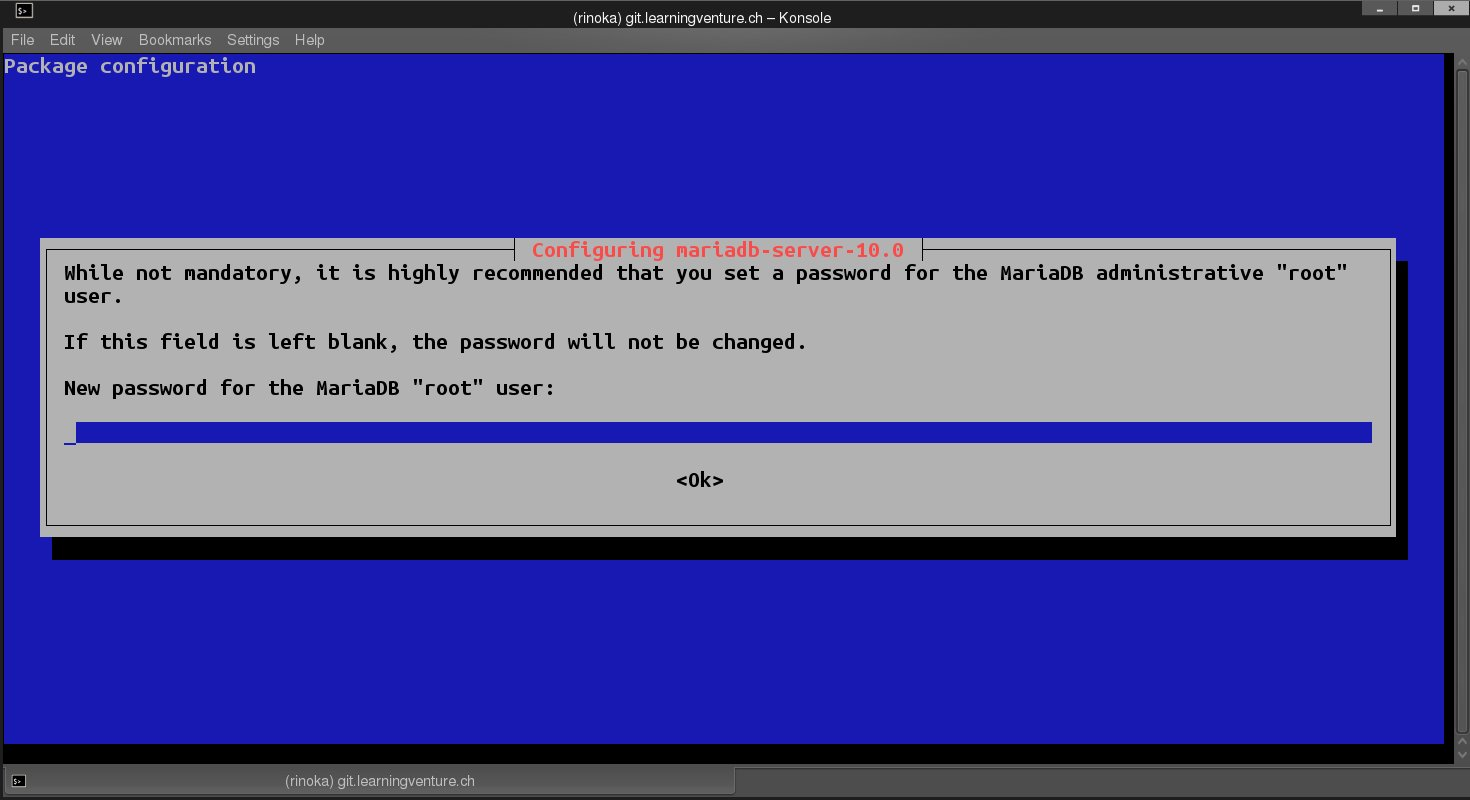
\includegraphics[width=13cm]{../Pics/3-lamp-stack-mariadb}
	Abbildung 1: Festlegung des Passworts für MariaDB-root
	\newline
	\newline
	Nach erfolgreichem Festlegen des Passworts für den MariaDB-root-user schliesst sich das Fenster wieder. Das Einrichten der Datenbank besprechen wir in der Sektion MariaDB.
	\subsection{Apache}
	Gemäss der im Auftrag erfordlichen Konfigurationsdateien muss die Wordpress-Installation auf dem Server unter /var/www/html/wordpress installiert werden.
	Allerdings soll Wordpress auf IP-Adresse/blog aufgerufen werden. Dazu muss der VirtualHost in /etc/apache2/sites-available/ angepasst werden.
	\subsubsection{VirtualHost}
	Die VirtualHost-Konfigurationsdatei befindet sich in /etc/apache2/sites-available/
	Darin befindet sich am Anfang eine Standard-Konfigurationsdatei mit dem Namen:
	\begin{itemize}
		\item 000-default.conf
	\end{itemize}		
	Die im Auftrag angegebene Konfigurationsdatei soll wordpress.conf heissen. Dazu könnten wir einfach die bestehende Datei umbenennen (mv 000-default.conf wordpress.conf), aber wir haben uns entschieden, sie beizubehalten und einfach basierend auf der Default-Datei eine entsprechende wordpress.conf zu erstellen (cp 000-default.conf wordpress.conf). Wichtig ist nun zu beachten, dass nicht beide Konfigurationsdateien aktiviert sind. Um das zu testen, untersucht man den Ordner sites-enabled wie folgt:
	\begin{itemize}
		\item ls /etc/apache2/sites-enabled
	\end{itemize}
	Falls sich  000-default.conf darin befindet, deaktiviert man sie folgendermassen:
	\begin{itemize}
		\item a2dissite  000-default.conf
	\end{itemize}
	Der Grund dafür ist, wenn beide Konfigurationsdateien aktiviert sind (d.h. 000-default.conf und wordpress.conf), dann wird nur 000-default.conf verwendet, weil sie alphabetisch vor wordpress.conf kommt (das kann man testen, wenn man 000-default.conf deaktiviert und in sites-available folgendermassen umbenennt: x000-default.conf). Wenn man x000-default.conf und wordpress.conf beide aktiviert, wird dieses mal wordpress.conf verwendet, weil w vor x kommt (diese möchten wir nur am Rande anmerken, weil wir uns beim Testen kurz mit dieser Situation auseinandersetzen mussten).
	\newline
	\newline
	Dazu möchten wir noch anmerken, dass dies allerdings nicht eintreffen sollte, wenn man einen Server mit Domain Name hat (z.B www.meinserver.ch) und einer entsprechend (gleich) benannten VHost.conf Datei (dem erwähnten Beispiel hier: meinserver.ch.conf). 
	\newline
	\newline
	Wie bereits erwähnt soll die Wordpress-Installation auf dem Server unter dem Dateipfad /var/www/html/wordpress erfolgen, allerdings mit IP-Adresse/blog erreichbar sein. Das funktioniert ohne entsprechende Anpassung in der VHost-Konfigurationsdatei allerdings nicht, weil was nach der IP-Adresse folgt, ist der System-Pfad der auf den im DocumentRoot angebenen Pfad folgt. Wenn im DocumentRoot z.B. /var/www/html steht, wird unsere Wordpress-Seite automatisch über IP-Adresse/wordpress zu erreichen sein, weil sie sich im Verzeichnis /var/www/html/wordpress befindet (also im DocumentRoot /var/www/html).
	\newline
	\newline
	Zur Lösung dieses Problems verwenden wir gemäss Dokumentation \url{https://httpd.apache.org/docs/2.2/mod/mod_alias.html\#alias} ein sogenanntes \textit{Alias}. Die Idee ist folgende:
	\begin{displayquote}
	The directives contained in this module allow for manipulation and control of URLs as requests arrive at the server. The \underline{Alias} and \underline{ScriptAlias} directives are used to map between URLs and filesystem paths.
	\end{displayquote}
	Das heisst, man kann mit einer bestimmten URL (in unserem Falle IP-adresse/blog) auf einen bestimmten Pfad auf dem Server selbst zugreifen (in unserem Falle /var/www/html/wordpress). Dazu muss die VirtualHost- Konfigurationsdatei in /etc/apache2/sites-available/wordpress.conf entsprechend angepasst werden:
	\newline
	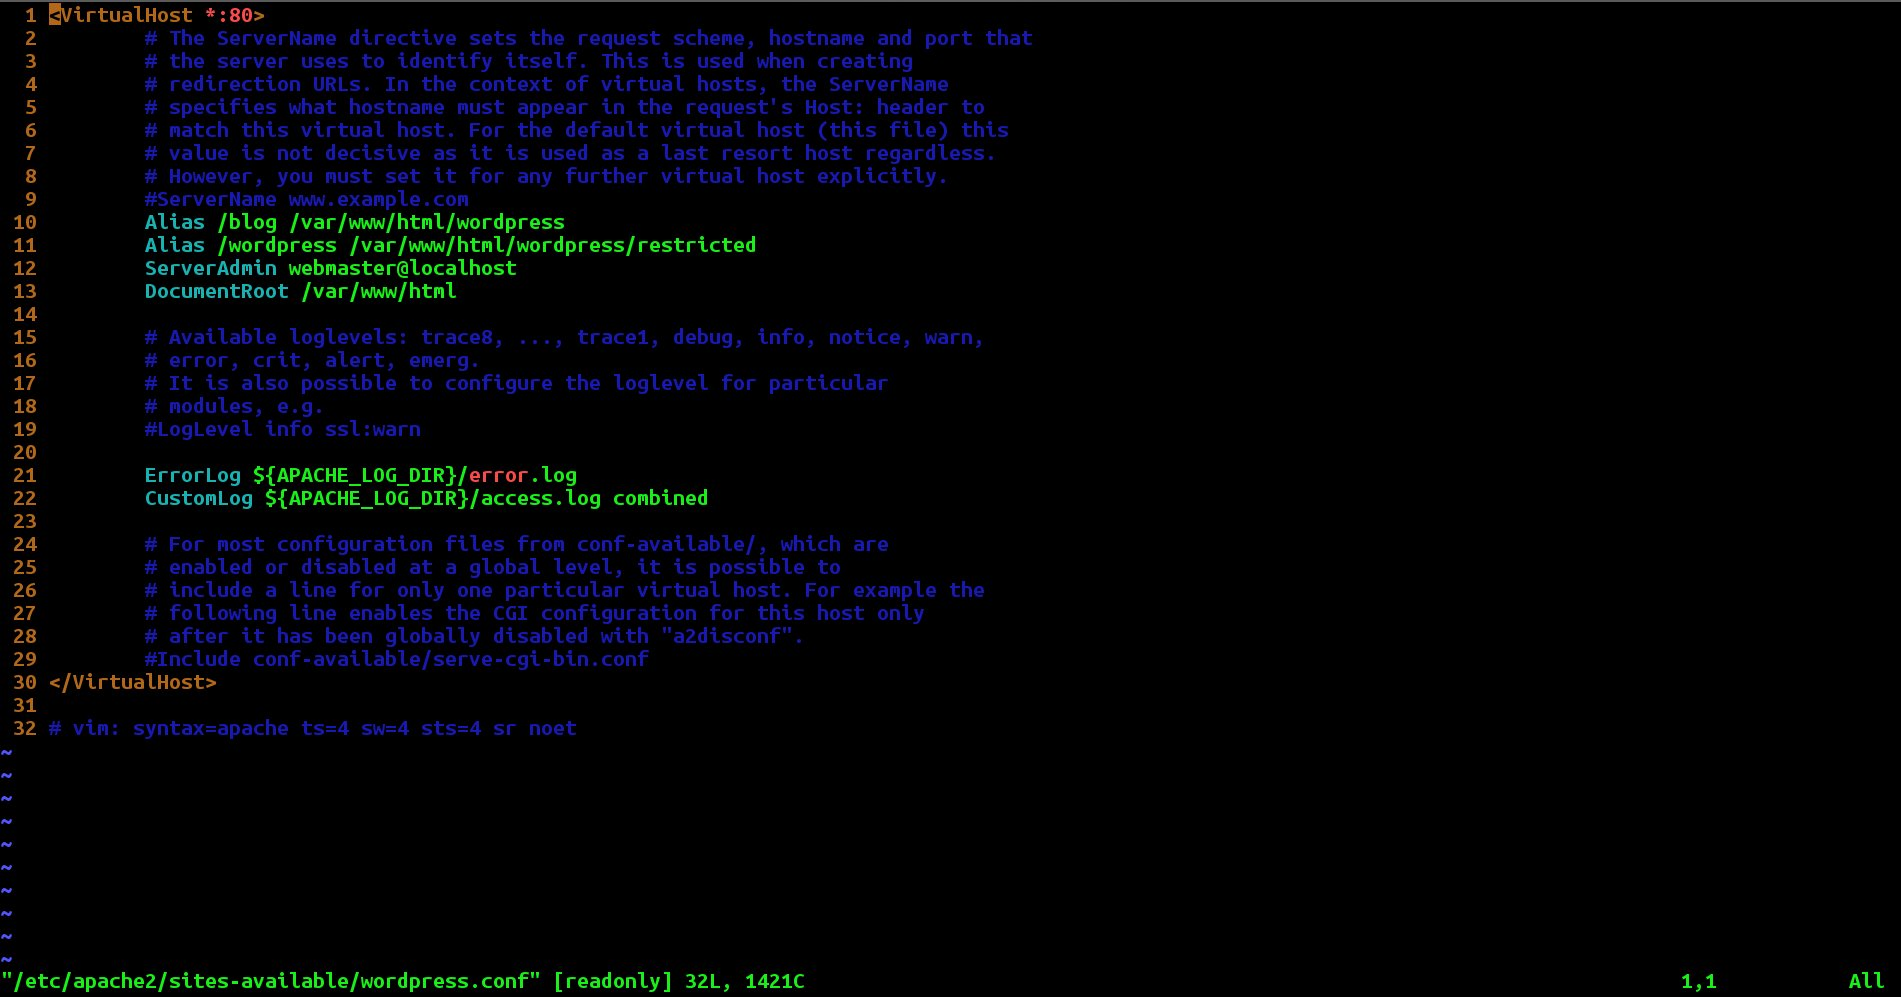
\includegraphics[width=13cm]{../Pics/wordpress}
	Abbildung 2: VHost-Datei in /etc/apache2/sites-available
	\newline
	\newline
	Dieses Alias wird der VirtualHost Konfigurations-Datei
	\newline
	/etc/apache2/sites-available/wordpress.conf hinzugefügt. Der Inhalt ist in Abbildung 2 zu sehen. Zusätzlich haben wir beschlossen, dass die
    \newline IP-Adresse/wordpress nicht auf den Blog führen soll (es reicht, wenn man über /blog drauf kommt). Zu diesem Zweck haben wir eine index.html mit einer kleinen Nachricht definiert. Schliesslich ist zu erwähnen, dass wir unsere VHost-Datei auf das Wesentliche beschränkt haben, d.h. wir haben sie nur mit dem für die zur Erfüllung der Aufgabe erfordlichen Inhalt bestückt.
	
	\subsection{MariaDB}
	Weil wir für Wordpress eine Datenbank brauchen, haben wir uns wie bereits erwähnt für \textit{\textbf{MariaDB}} als Datenbank entschieden und wie bereits in der LAMP-Sektion beschrieben installiert sowie ein Passwort für den root user der MariaDB festgelegt. Nun kümmern wir uns um die Einrichtung.
	\newline
	\newline
	Zunächst einmal müssen wir uns einloggen, das machen wir mit folgendem befehl:
	\begin{lstlisting}[language=bash]
	# mysql -u root -p
	\end{lstlisting}
	Nach erfolgreicher Ausführung sehen wir Folgendes:
	\newline
	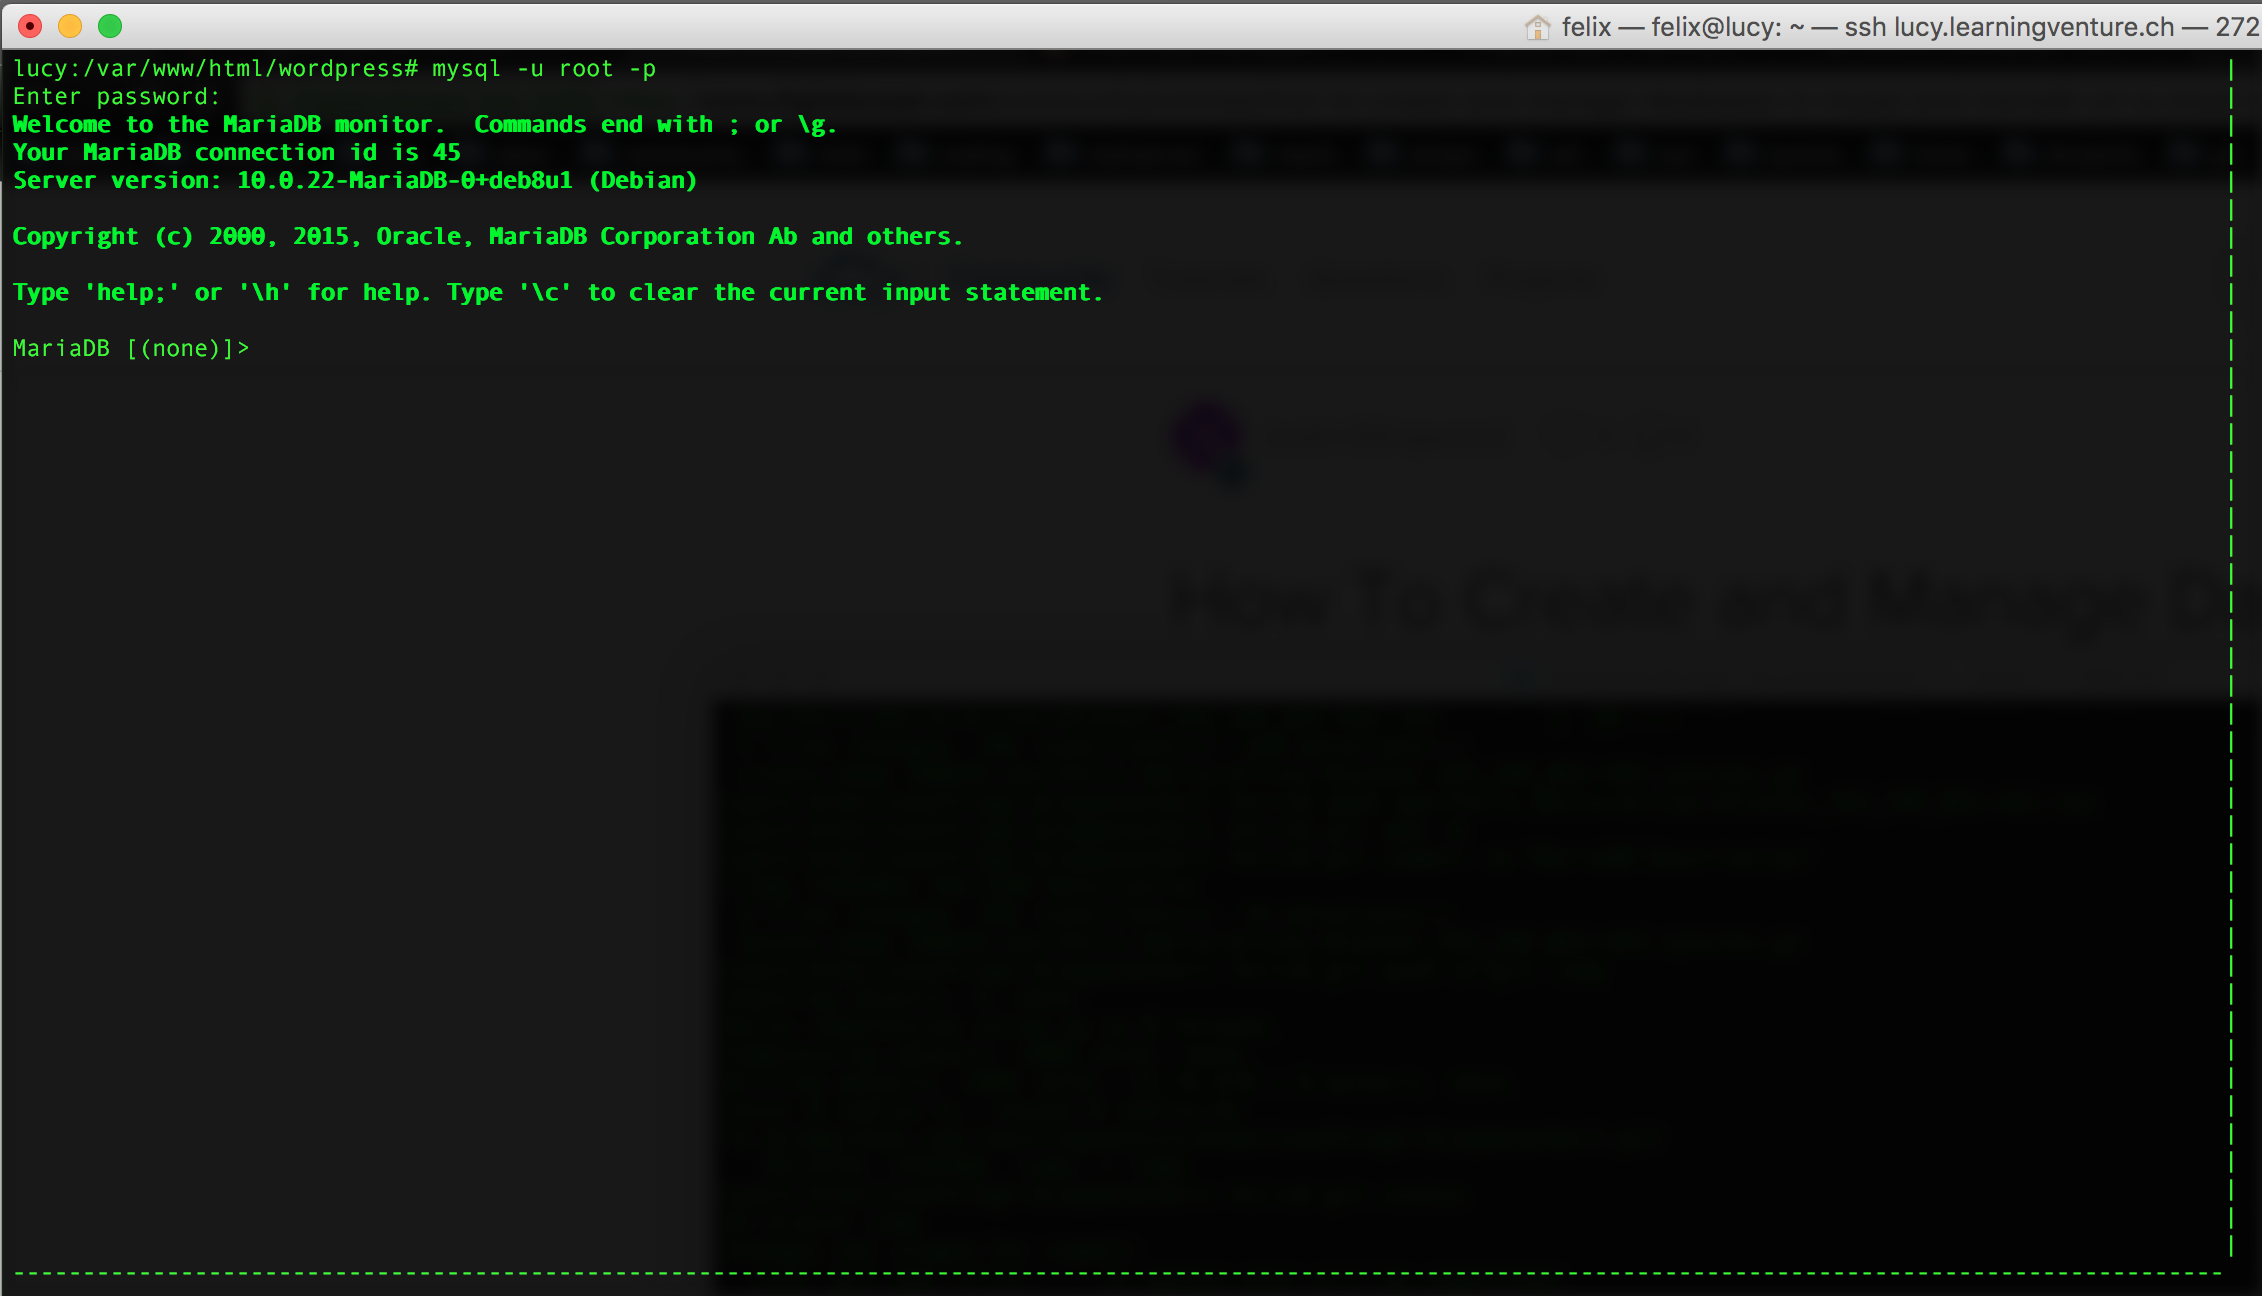
\includegraphics[width=13cm]{../Pics/21-maria-db-login-success}
	Abbildung 3: Login MariaDB
	\newline
	\newline
	Nun können wir die eigentliche Datenbank erstellen. Das machen wir mit dem in Abbildung 4 dargestellten Befehl:
	\newline
	\newline
	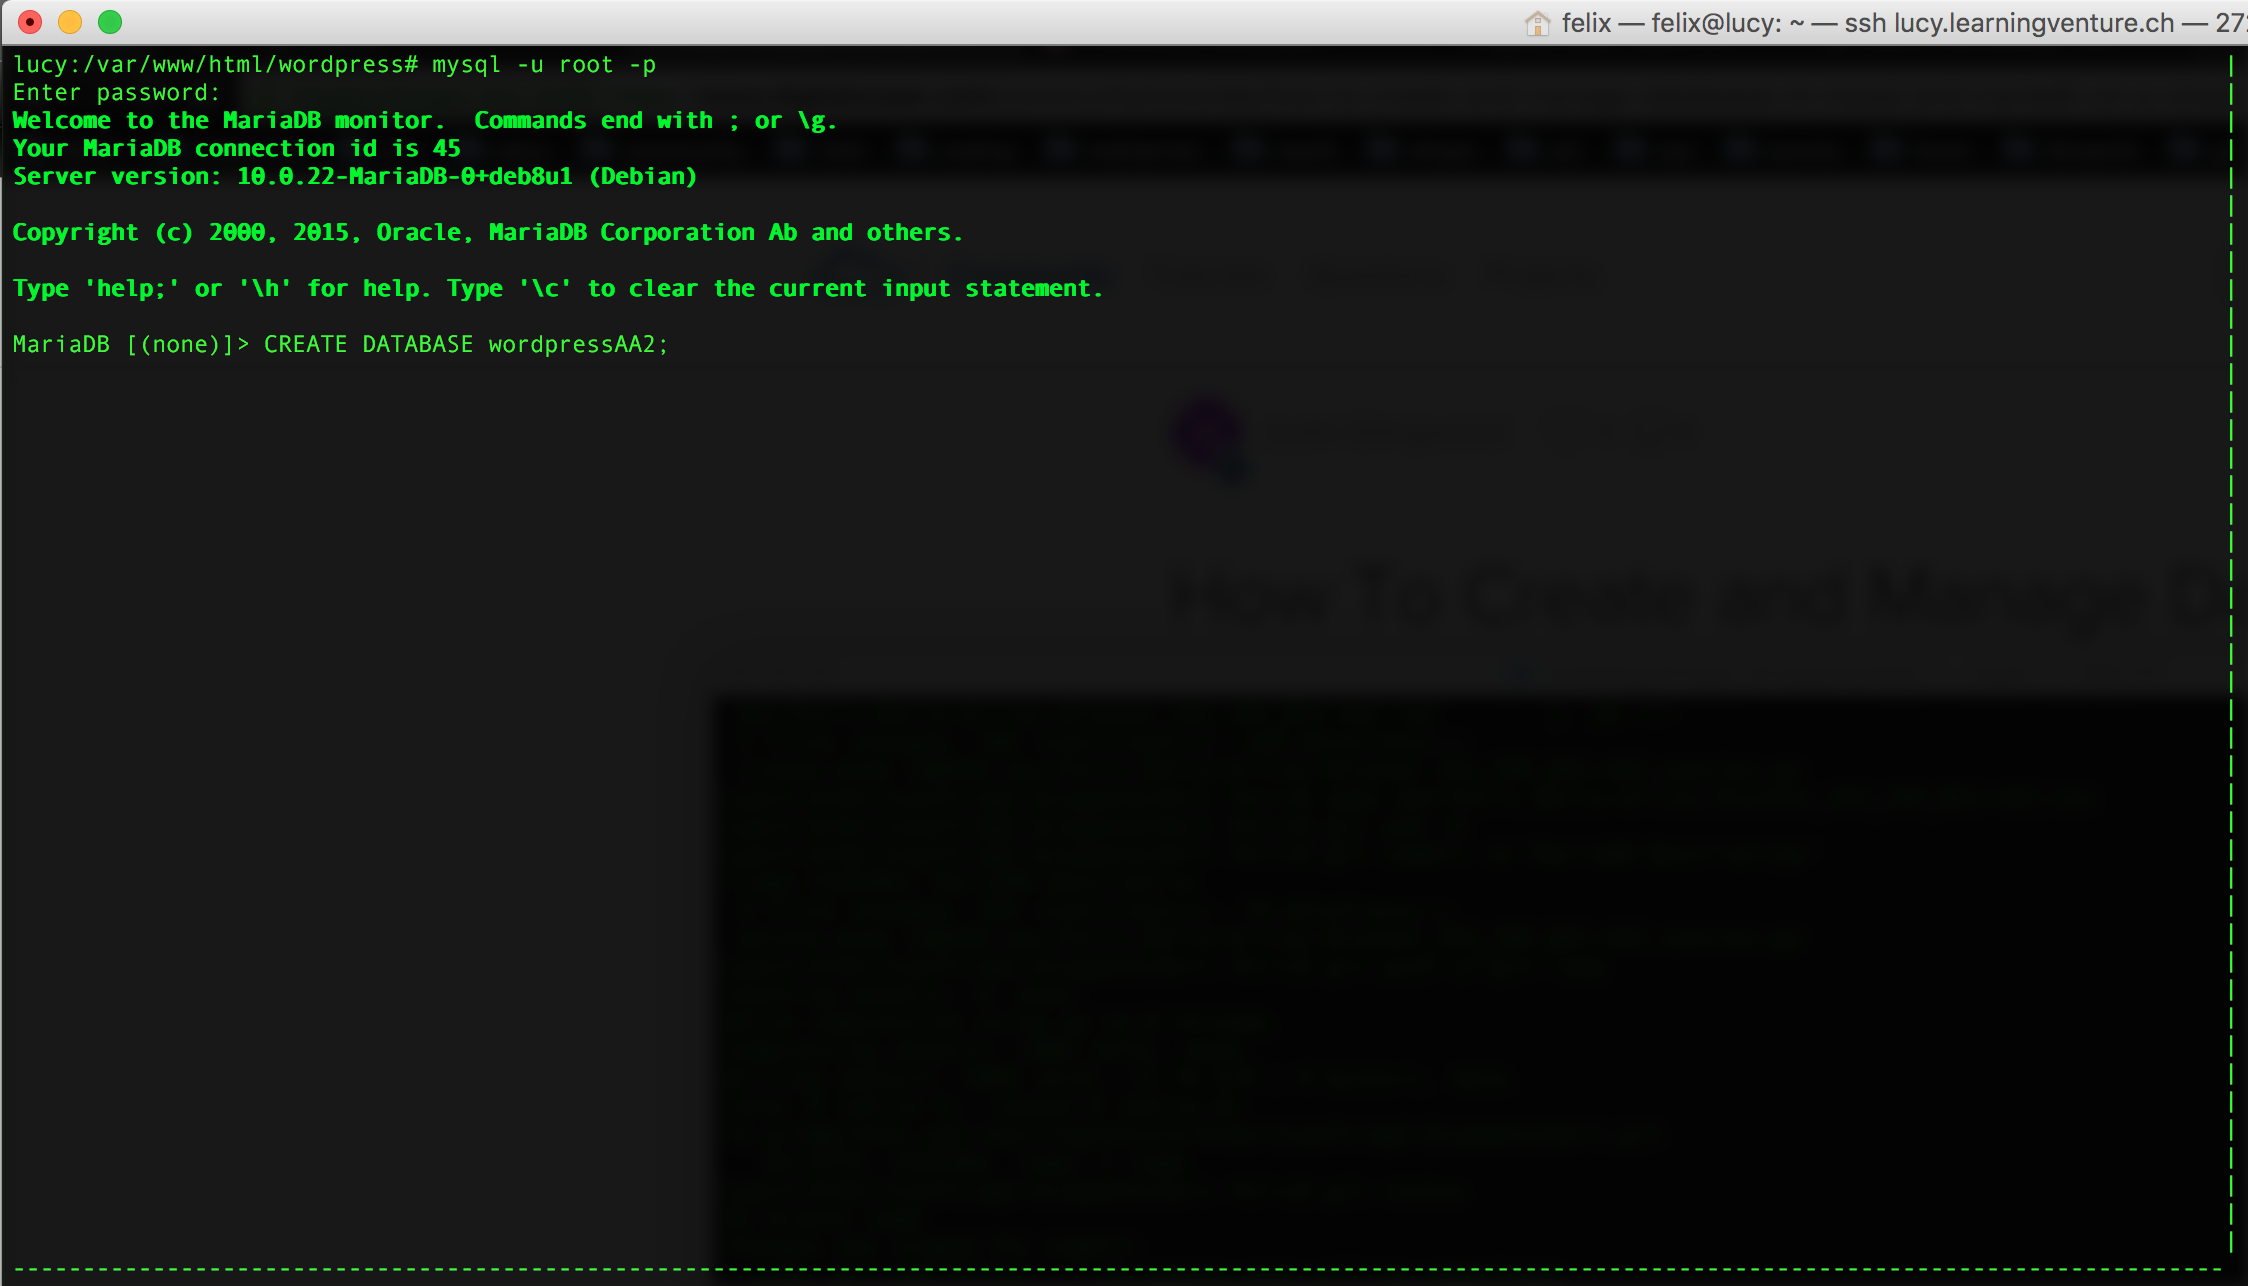
\includegraphics[width=13cm]{../Pics/22-maria-db-create}
	Abbildung 4: Erstellung einer Datenbank mit CREATE DATABASE
	\newline
	\newline
	Wenn diese erfolgreiche erstellt wurde:
	\newline
	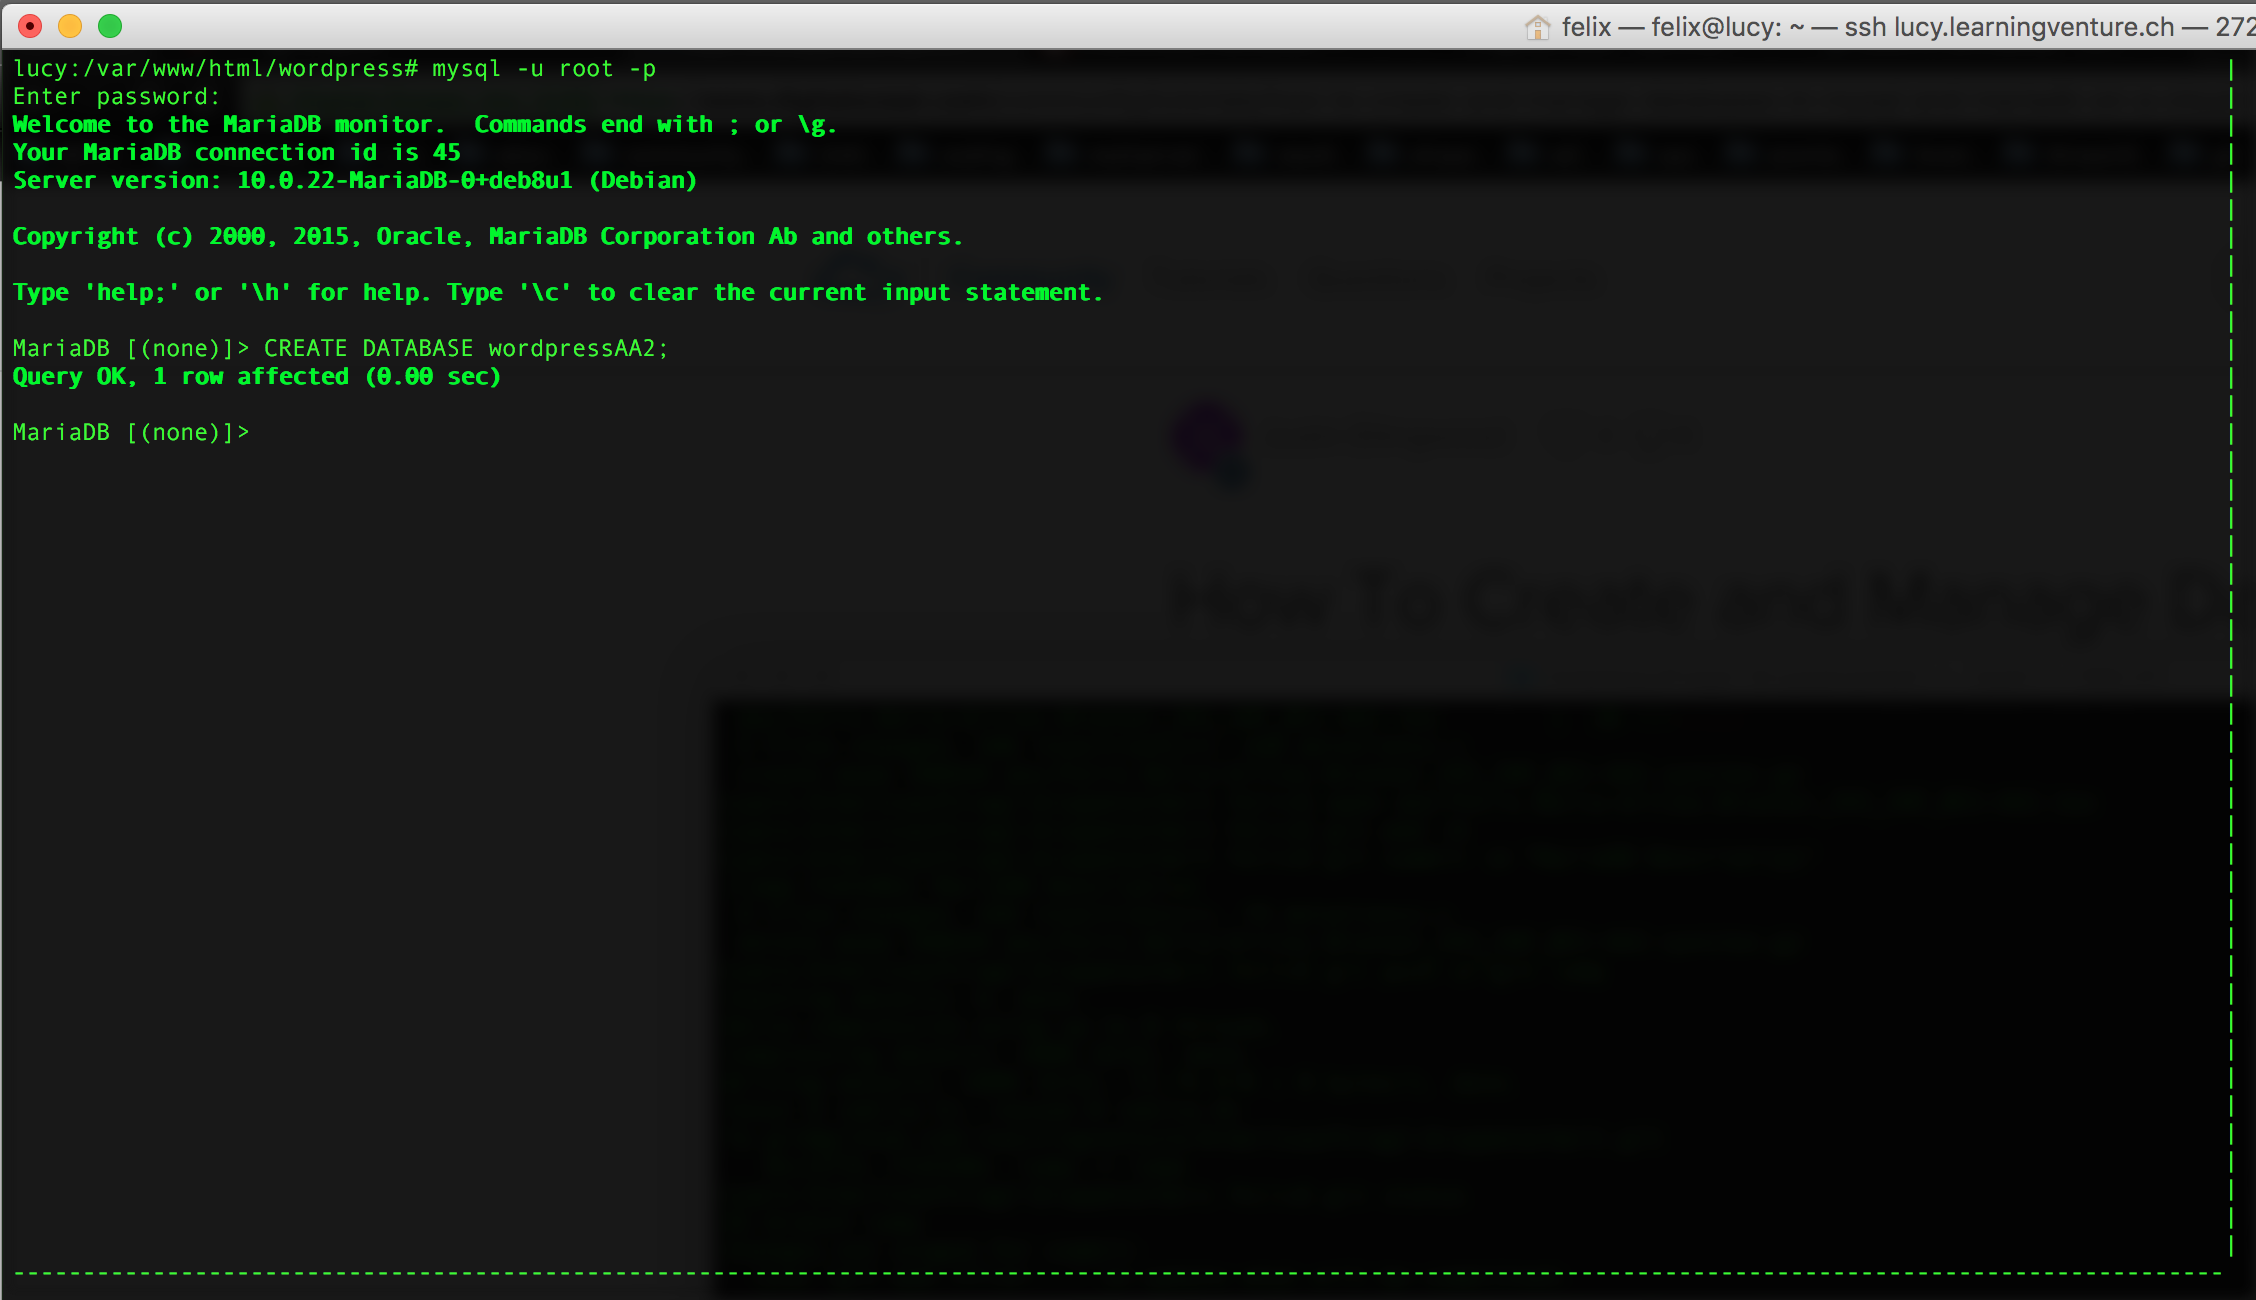
\includegraphics[width=13cm]{../Pics/23-maria-db-create-success}
	Abbildung 5: Erfolgreiche Erstellung einer Datenbank
	\newline
	\newline
	Zur Kontrolle, ob die gewünschte Datenbank erstellt wurde, kann man den in Abbildung 6 verwendeten Befehl eingeben:
	\newline
	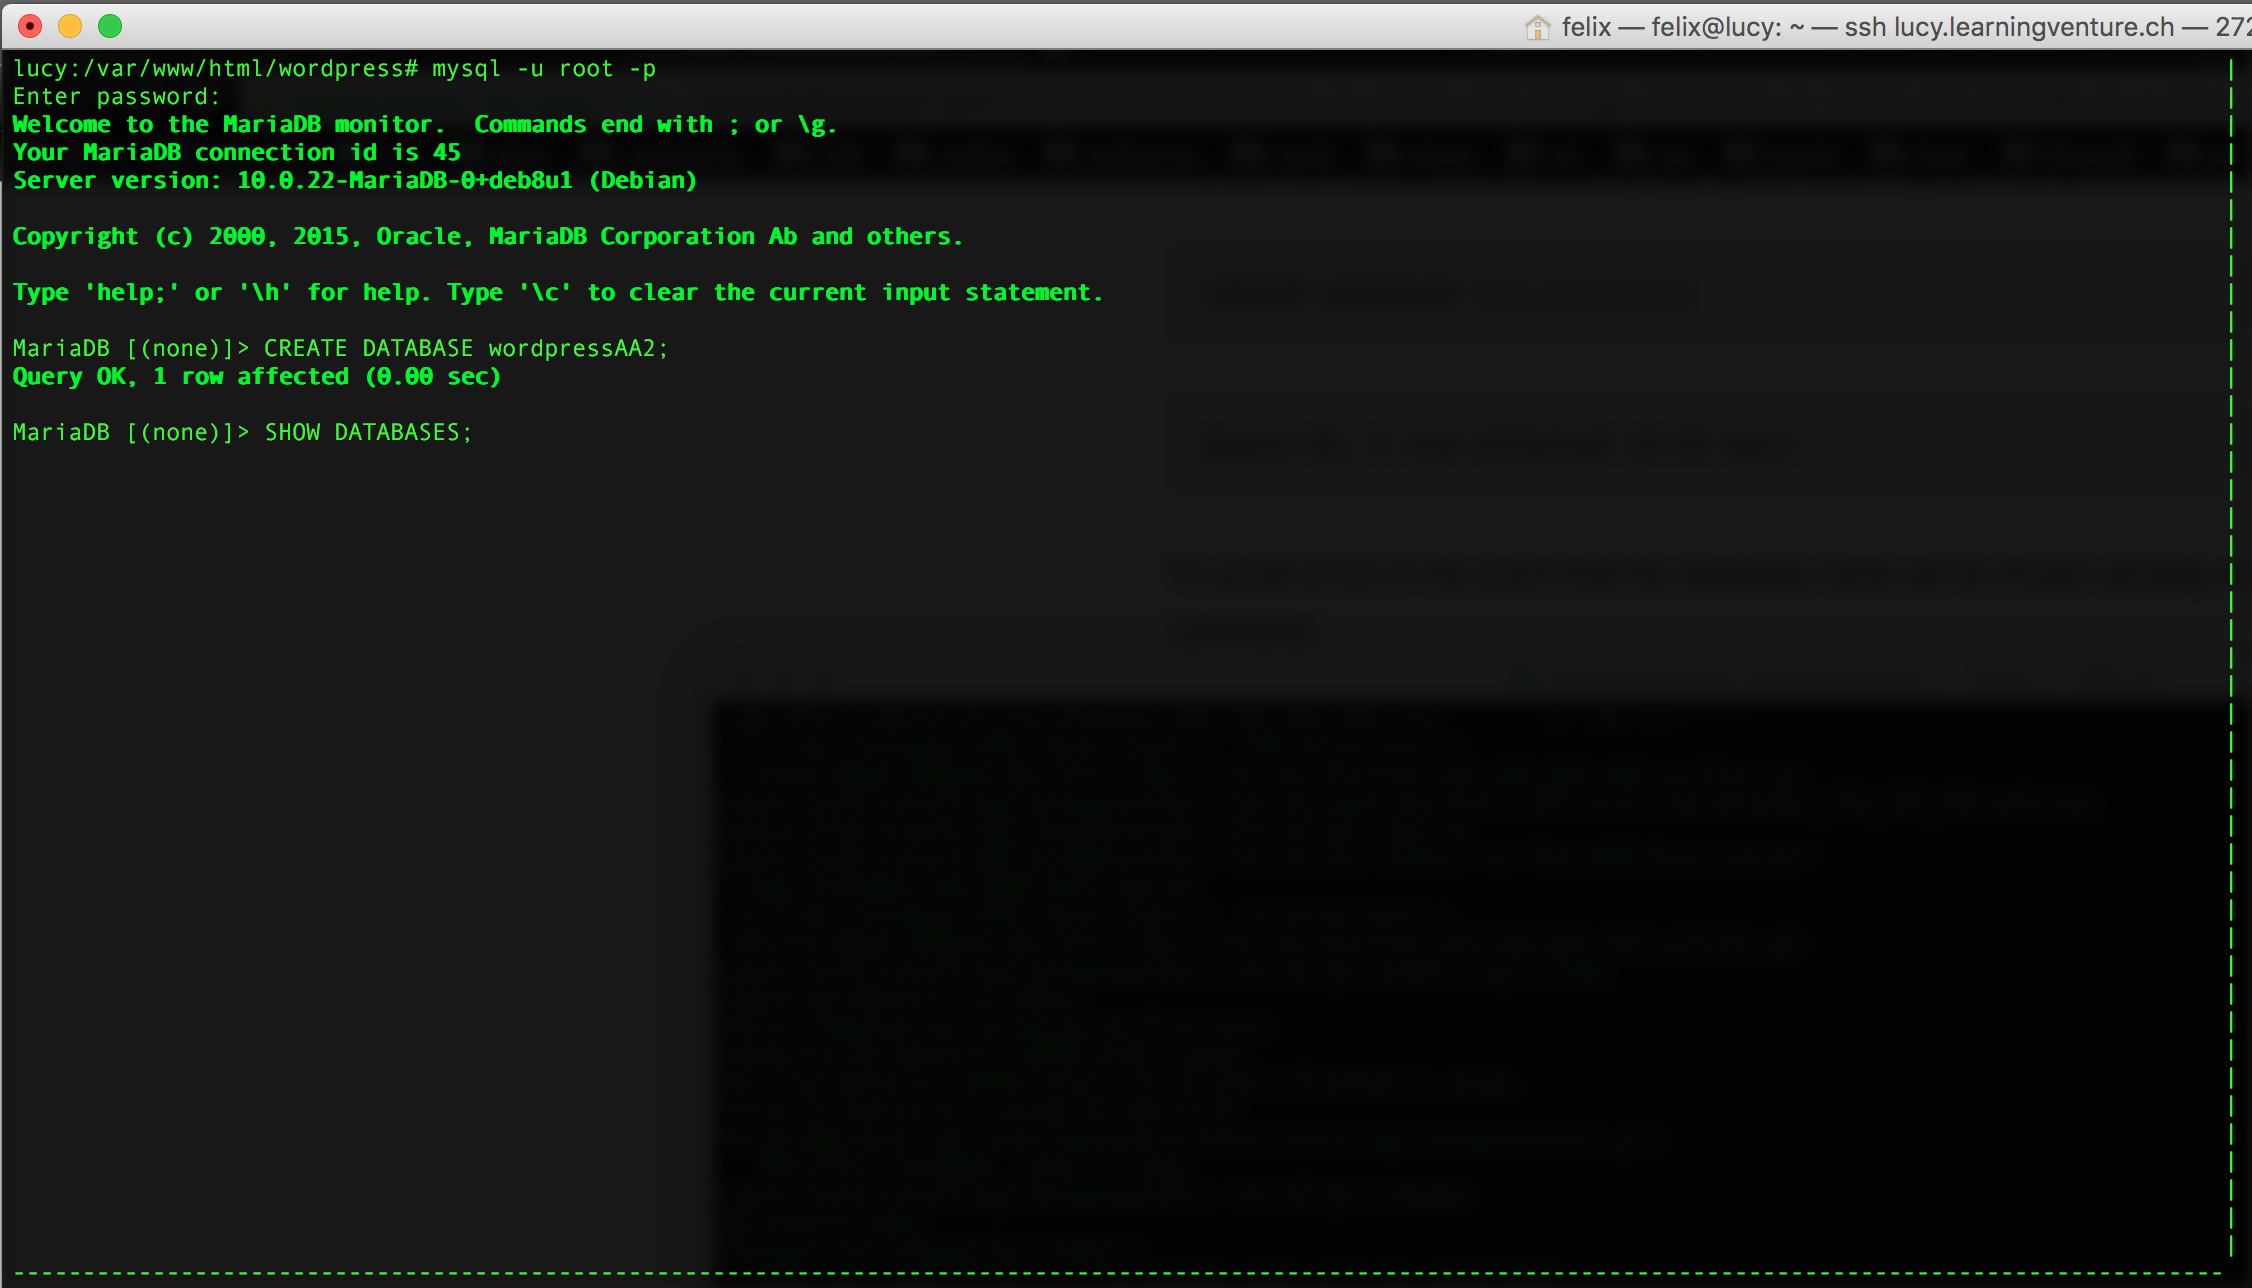
\includegraphics[width=13cm]{../Pics/24-maria-db-show}
	Abbildung 6: Kontrolle, ob Datenbank erfolgreich erstellt wurde
	\newline
	\newline
	Auf Abbildung 7 wird dargestellt, wie alles aussieht, wenn es korrekt ausgeführt wurde:
	\newline
	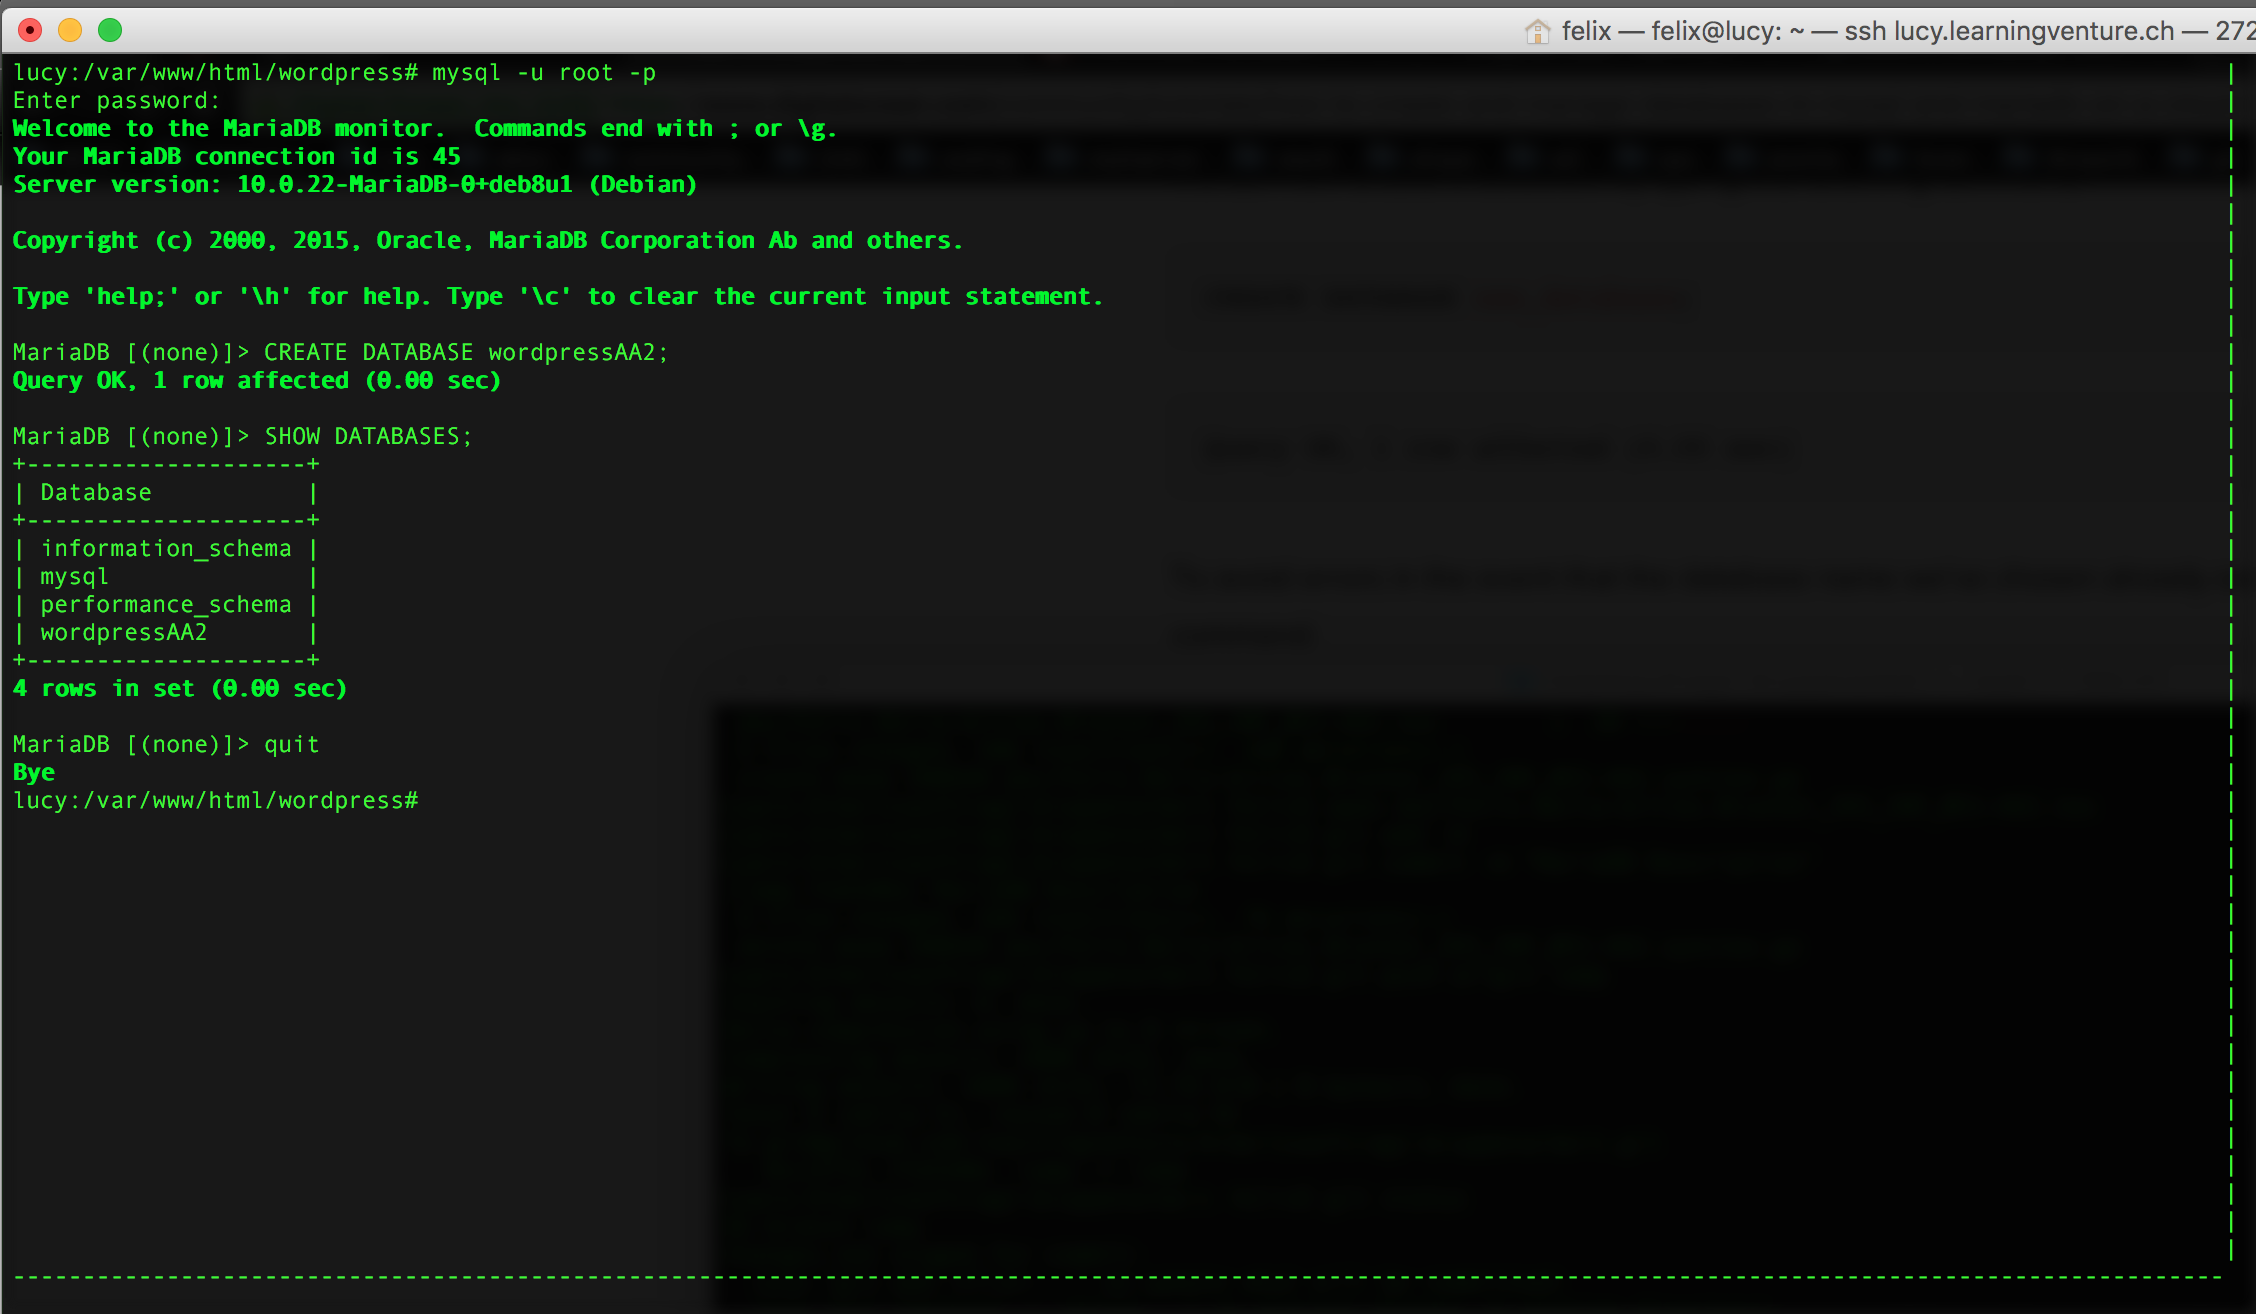
\includegraphics[width=13cm]{../Pics/27-maria-db-quit-success}
	Abbildung 7: Datenbank wordpressAA2 erfolgreich erstellt
	\newline
	\newline
	Nun kann man MariaDB mit dem Befehl \textit{quit} verlassen und sich um die Wordpress-Installation kümmern.
	
	\section{WordPress}
	Nach erfolgreichem Aufsetzen des LAMP-Stacks widmen wir uns in dieser Sektion der Installation und Konfiguration von Wordpress.
	\newline
	\newline
	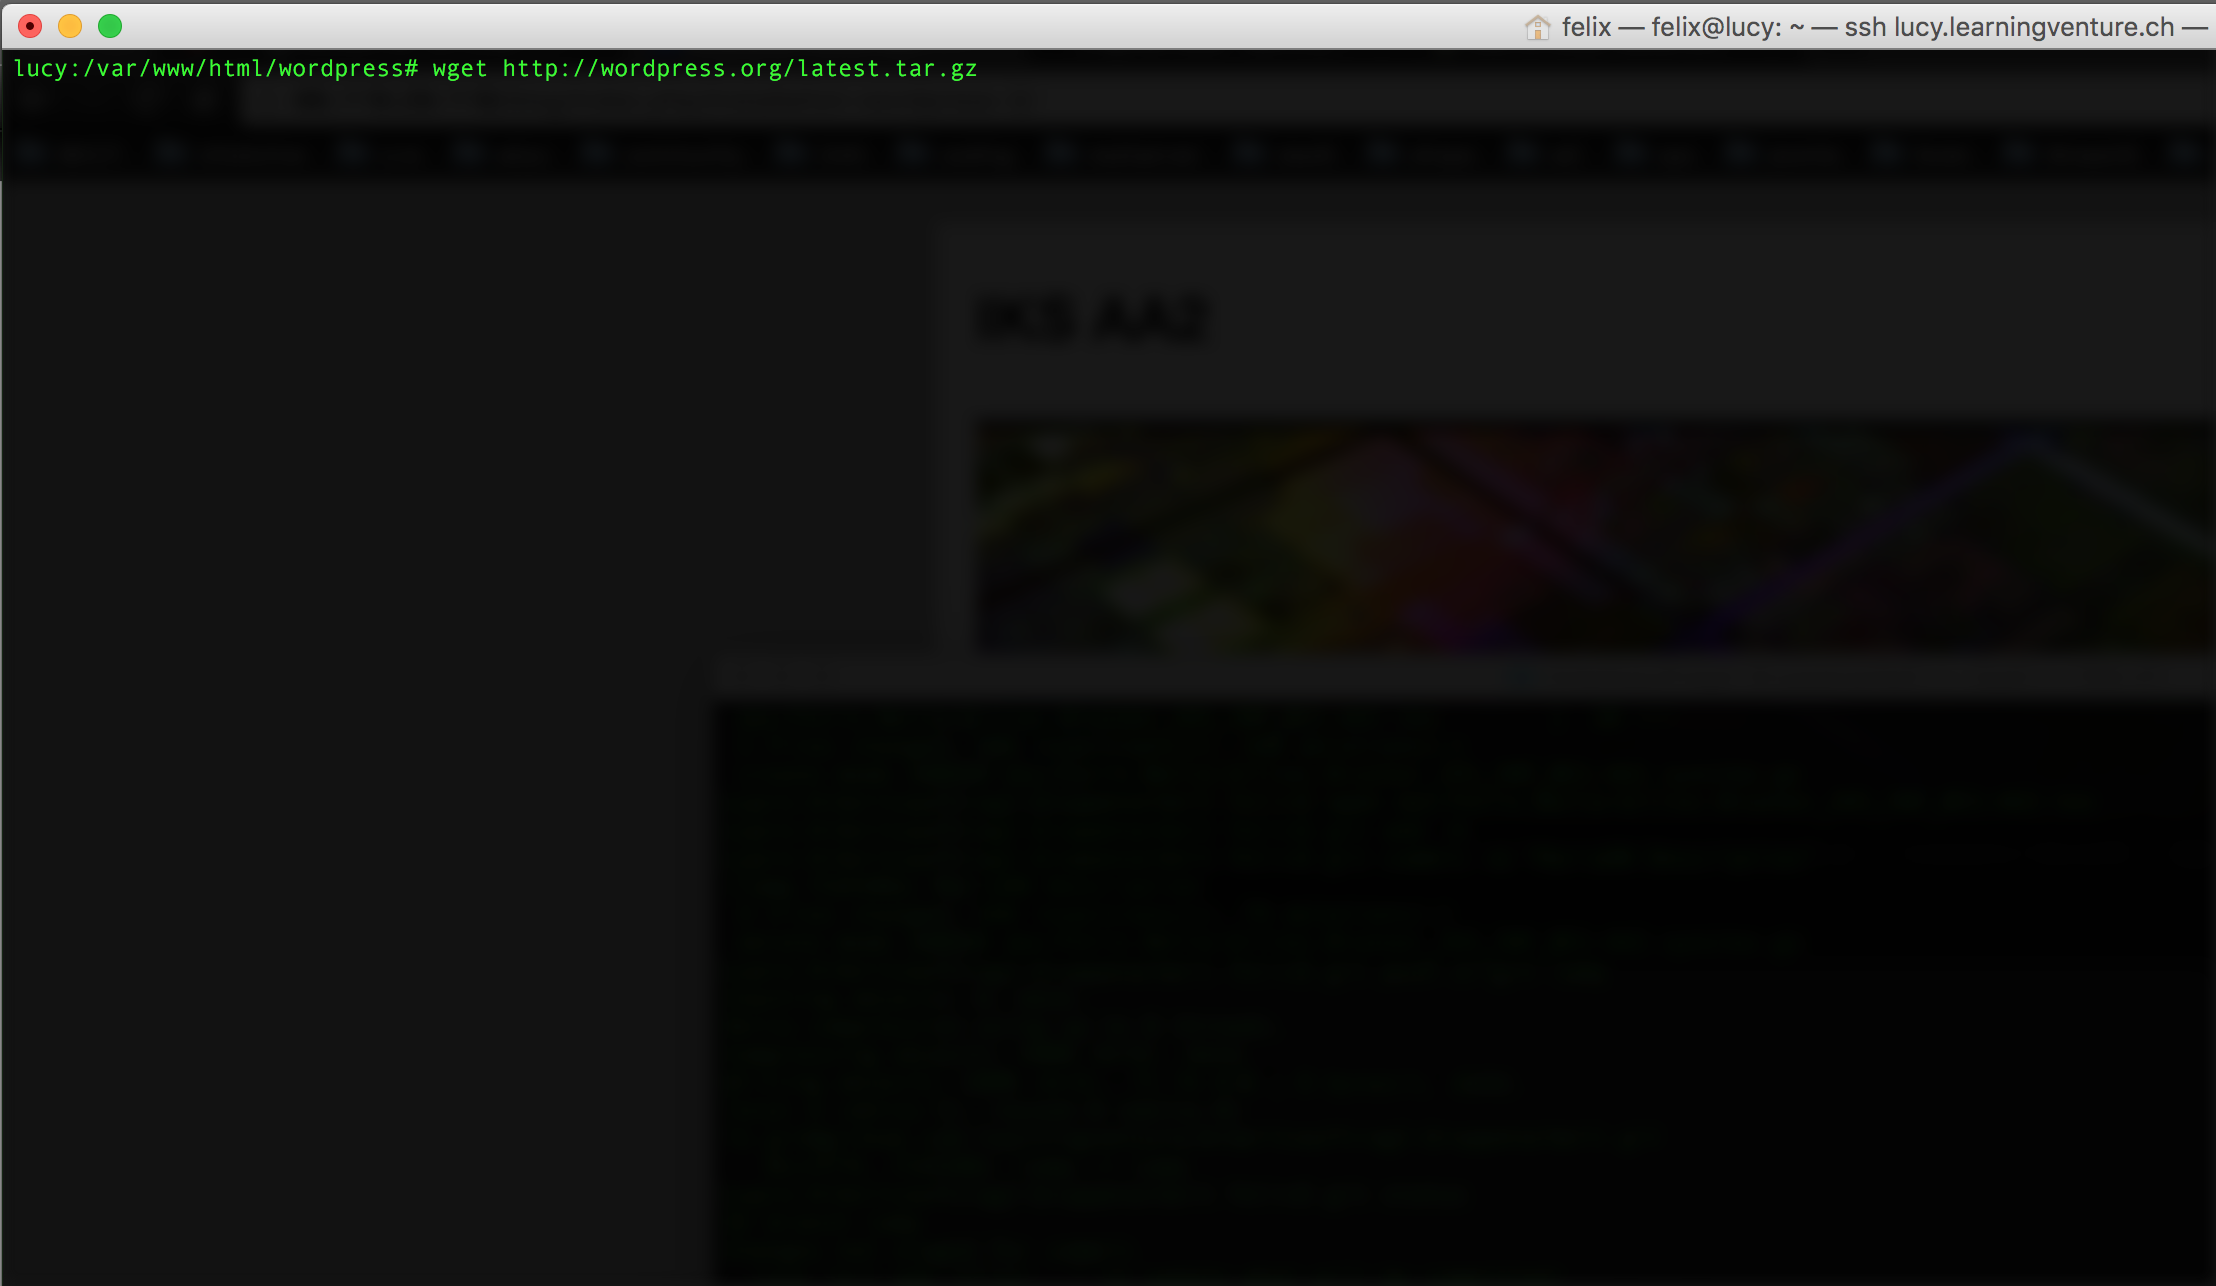
\includegraphics[width=13cm]{../Pics/30-wordpress-download}
	Abbildung 8: Download der neusten Wordpress-Version
	\newline
	\newline
	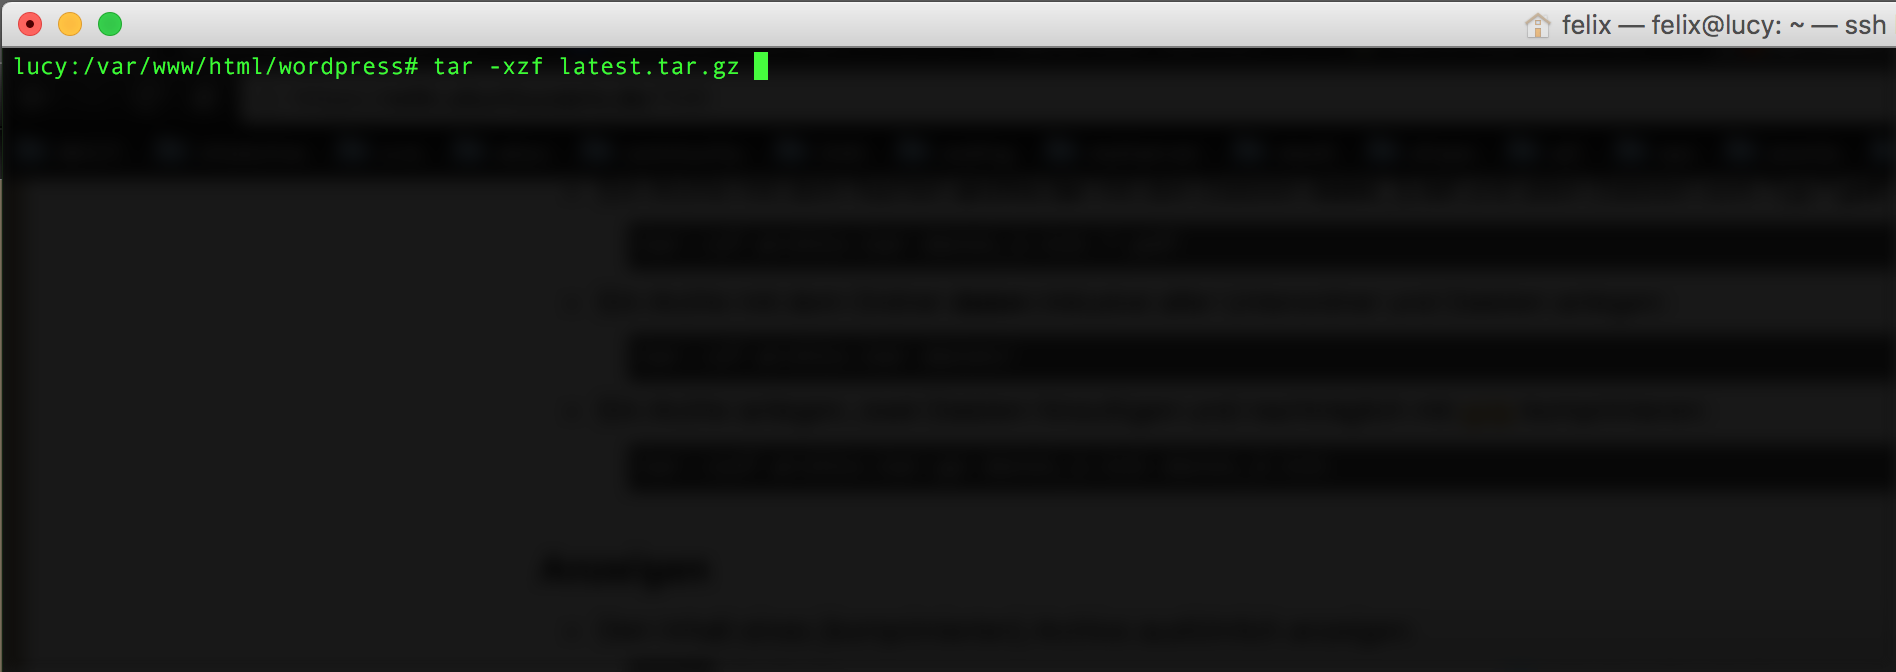
\includegraphics[width=13cm]{../Pics/32-wordpress-unzip}
	Abbildung 9: Befehl zum Entpacken der komprimierten Wordpress-Datei
	\newline
	\newline
	Nachdem Entpacken der Datei müssen wir zur korrekten Installation unseres Wordpress-Blogs ein paar Sachen vornehmen.
	\newline
	Wie in Abbildung 9 zu entnehmen ist, befinden wir uns beim Download bereits im Verzeichnis wordpress. Dieser Ordner existiert bereits, weil wir zu Testzwecken unseres Severs eine HTML-File in den Wordpress-Ordner gestellt haben. Im Normalfall würde man sich beim Downloaden der komprimierten WordPress-Datei im Verzeichnis /var/www/html befinden und beim Entpacken wird der Ordner \textit{wordpress} automatisch im Verzeichnis html entpackt. Da wir uns aber bereits im Verzeichnis /var/www/html/wordpress befinden, wird unsere WordPress-Installation in /var/www/html/wordpress/wordpress entpackt. Man kann die Dateien einfach eine Stufe herauf verschieben:
	\newline
	\begin{lstlisting}[language=bash]
	# mv * /var/www/html/wordpress/wordpress 
	  /var/www/html/wordpress
	\end{lstlisting}
	Die heruntergeladene Datei latest.tar.gz und den leeren Ordner /var/www/html/wordpress/wordpress kann man dann getrost mit der command rm entfernen:
	\begin{lstlisting}[language=bash]
	# rm /var/www/html/wordpress/latest.tar.gz
	\end{lstlisting}
	\begin{lstlisting}[language=bash]
	# rm -r /var/www/html/wordpress/wordpress
	\end{lstlisting}
	Da wir mit Root-Rechten arbeiten, kann es sein, dass die Berichtungen für den Apache-User beim WordPress-Ordner nicht richtig gesetzt sind. Ein Beispiel in Abbildung 10 mit dem Befehl ls sowie dem Befehl chown, um den Apache-User und die -Gruppe www-data Als Besitzer von Wordpress festzulegen:
	\newline
	\newline
	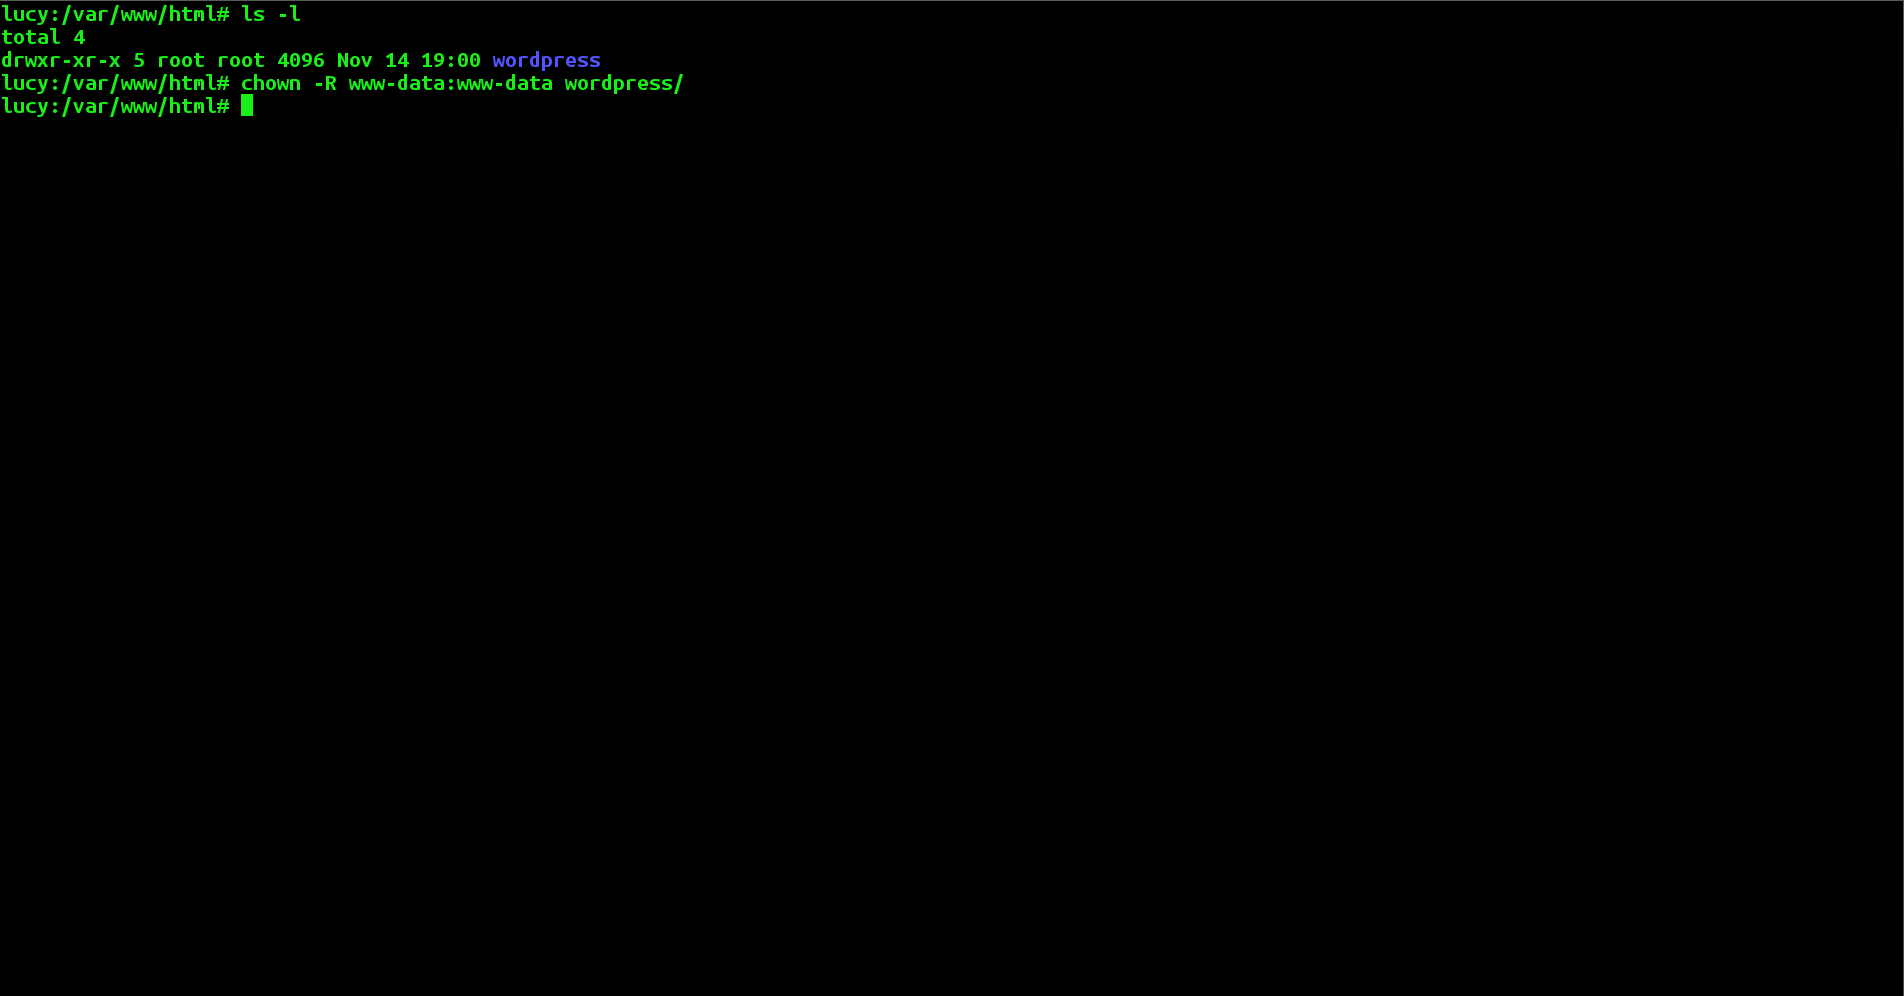
\includegraphics[width=13cm]{../Pics/35-wordpress-permissions}
	Abbildung 10: Ordner-Berechtigungen korrigieren.
	\newline
	\newline
	Nun sind wir soweit, unsere WordPress-Installtion im Web-Browser zu starten. Um sicher zu sein, dass dies auch klappt, kann man den Apache-Server mit folgendem Befehl neu starten:
	\begin{lstlisting}[language=bash]
	# service apache2 restart
	\end{lstlisting}
	Aufgrund der bisher gemachten Konfigurationen, geben wir im Web-Browser IP-Adresse/blog ein und landem auf folgendem Bildschirm:
	\newline
	\newline
	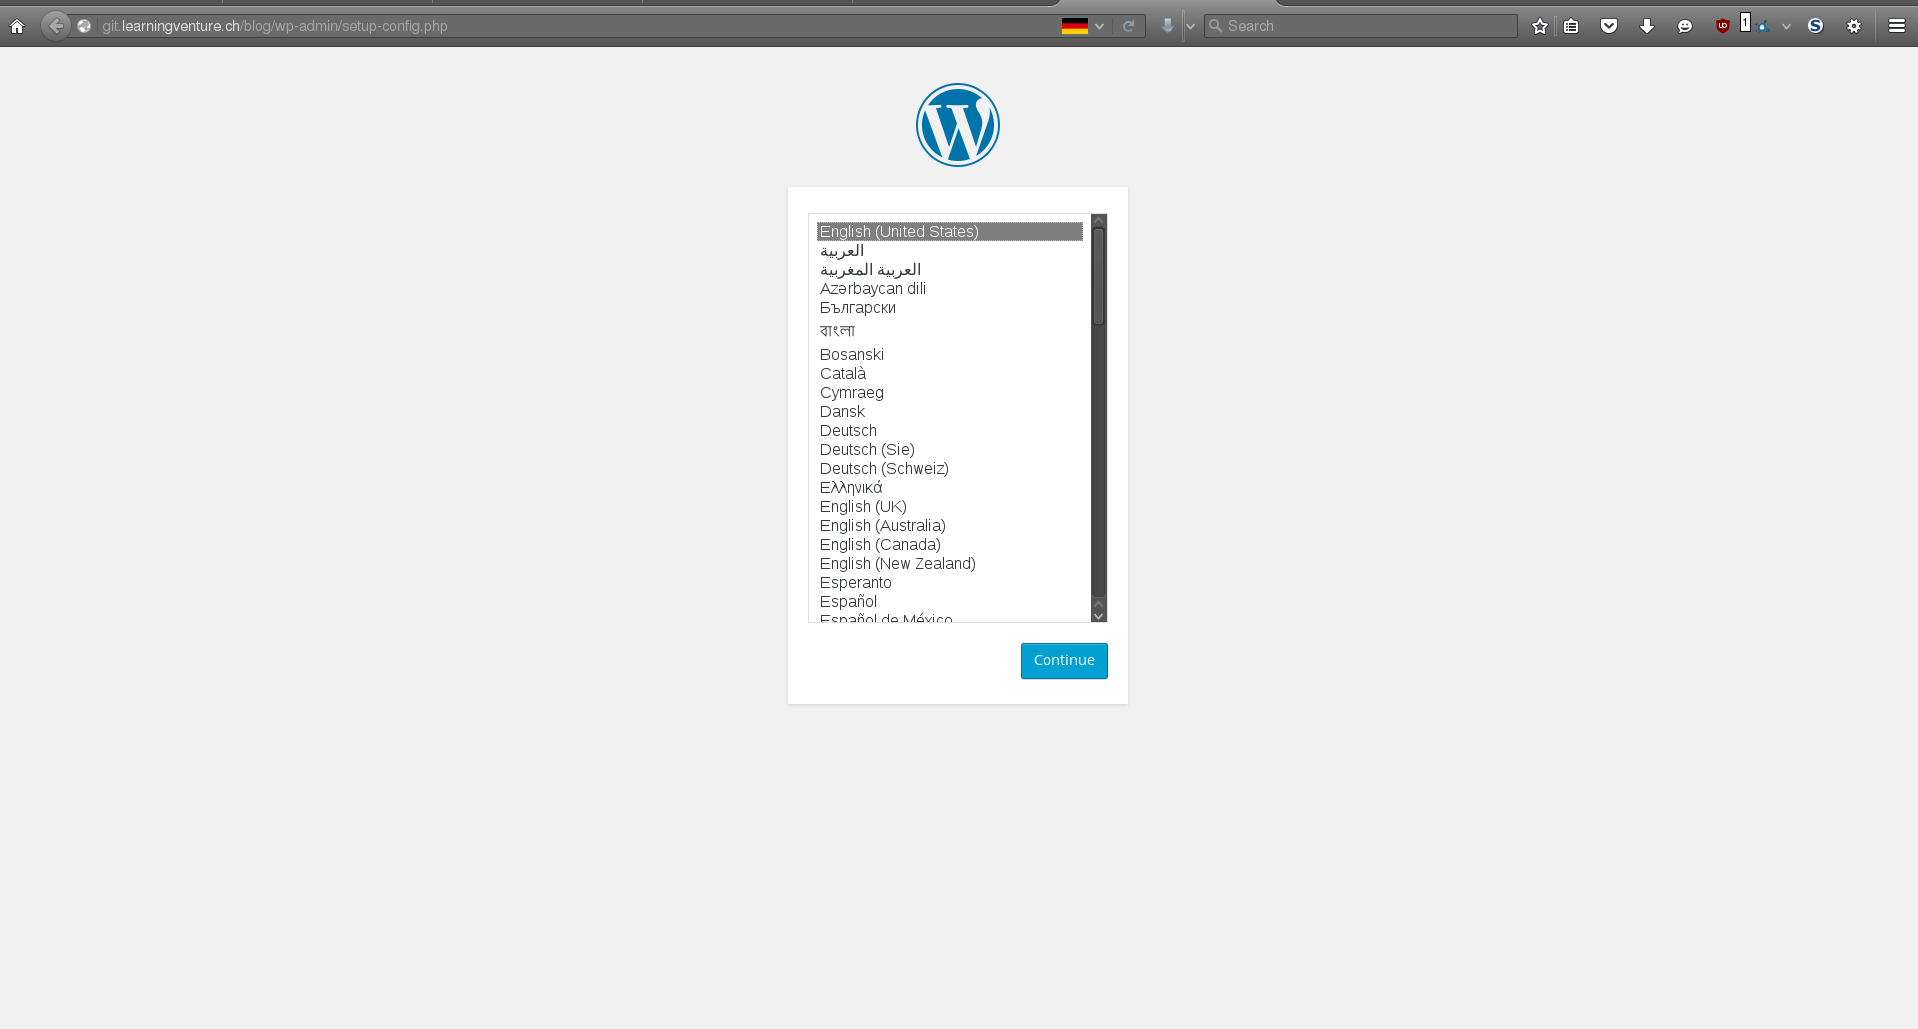
\includegraphics[width=13cm]{../Pics/36-wordpress-konfbildschirm}
	Abbildung 11: WordPress Spracheinstellung
	\newline
	\newline
	Dann kommen wir zum Bildschirm, wo wir Details für unsere Datenbank eintragen sollen. Dazu beziehen wir uns auf den Namen unserer MariaDB-Konfiguration:
	\begin{itemize}
	\item Datenbank Name: \textit{wordpressAA2}
	\end{itemize}
	\begin{itemize}
	\item Benutzername: \textit{root}
	\end{itemize}
	\begin{itemize}
	\item Passwort: \textit{das für den root gewählte Passwort}
	\end{itemize}
	\begin{itemize}
	\item Datenbankhost: \textit{localhost}
	\end{itemize}
	\begin{itemize}
	\item Tabellen-Präfix: \textit{wp}
	\end{itemize}
	Wenn alles erflogreich konfiguriert wurde, erscheint folgende Meldung:
	\newline
	\newline
	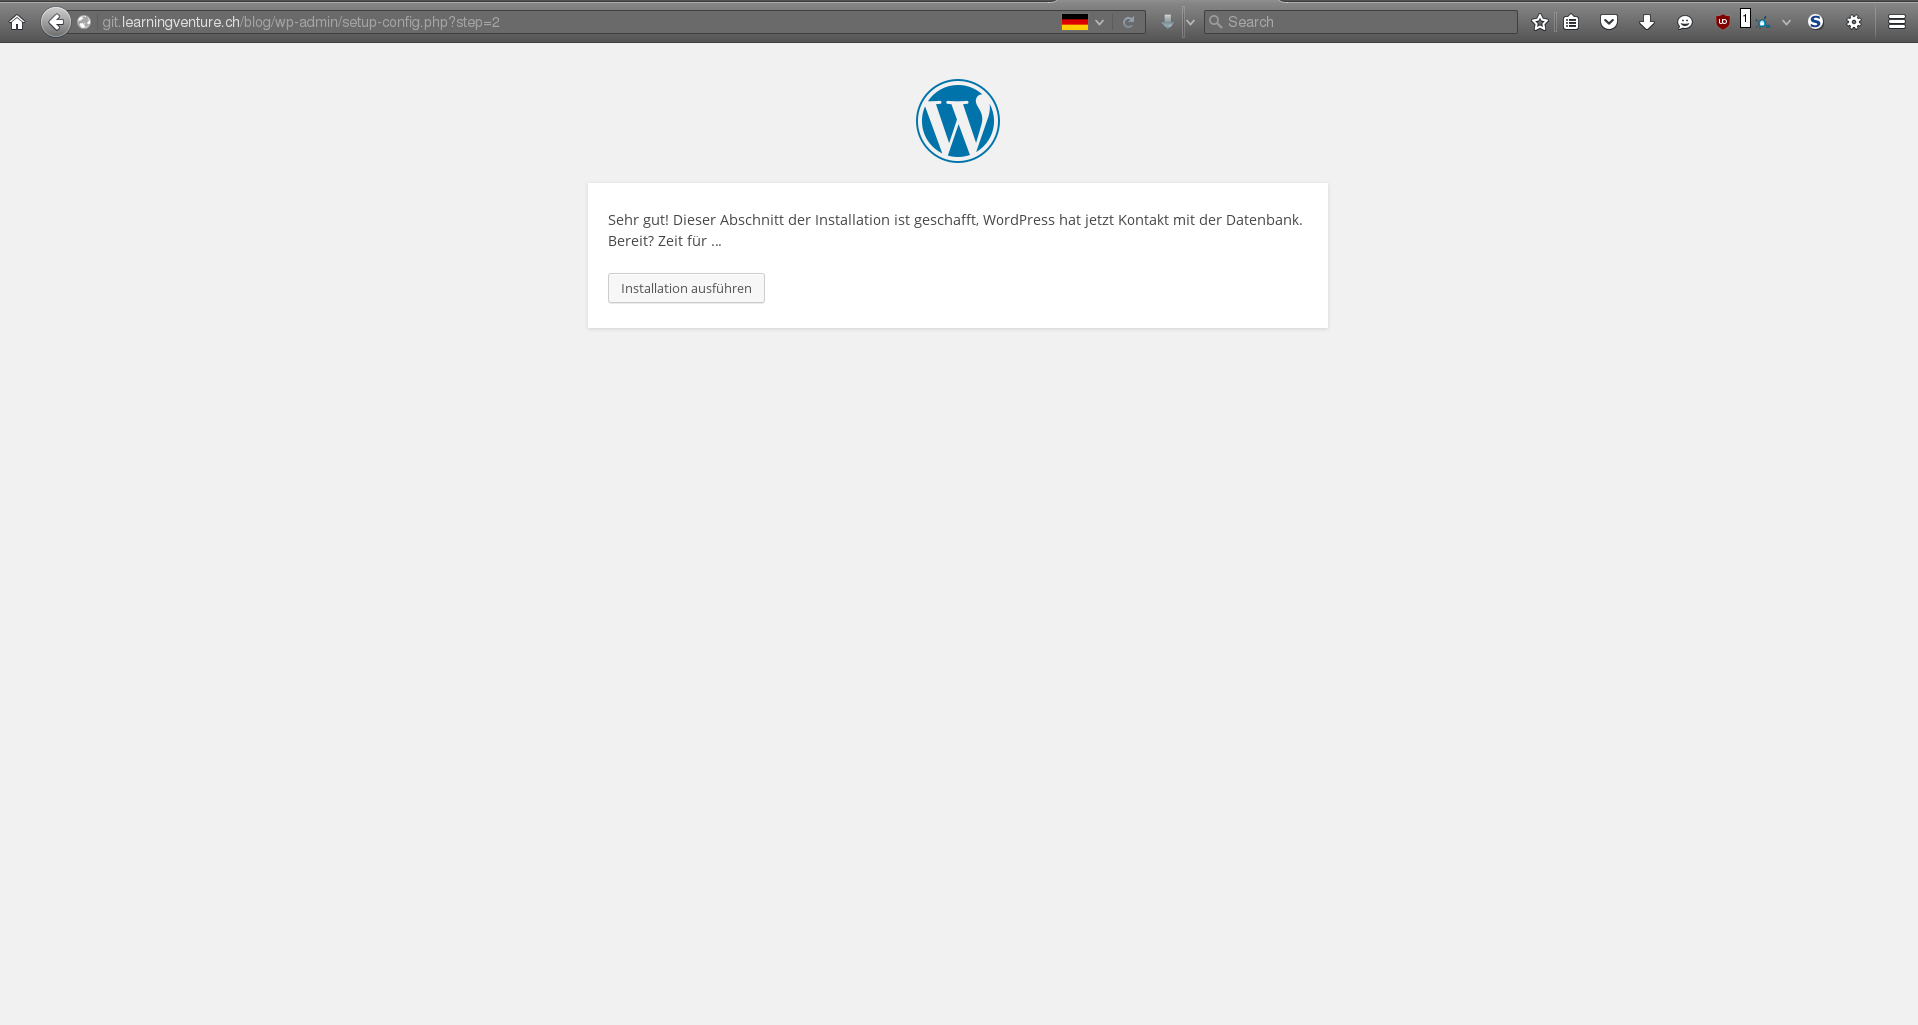
\includegraphics[width=13cm]{../Pics/37-wordpress-databas_ok}
	Abbildung 12: Datenbank erfolgreich konfiguriert.
	\newline
	\newline
	Die eigentliche WordPress-Installation haben wir ganz einfach wie in Abbildung 13 dargstellt ausgefüllt und abgeschlossen:
	\newline
	\newline
	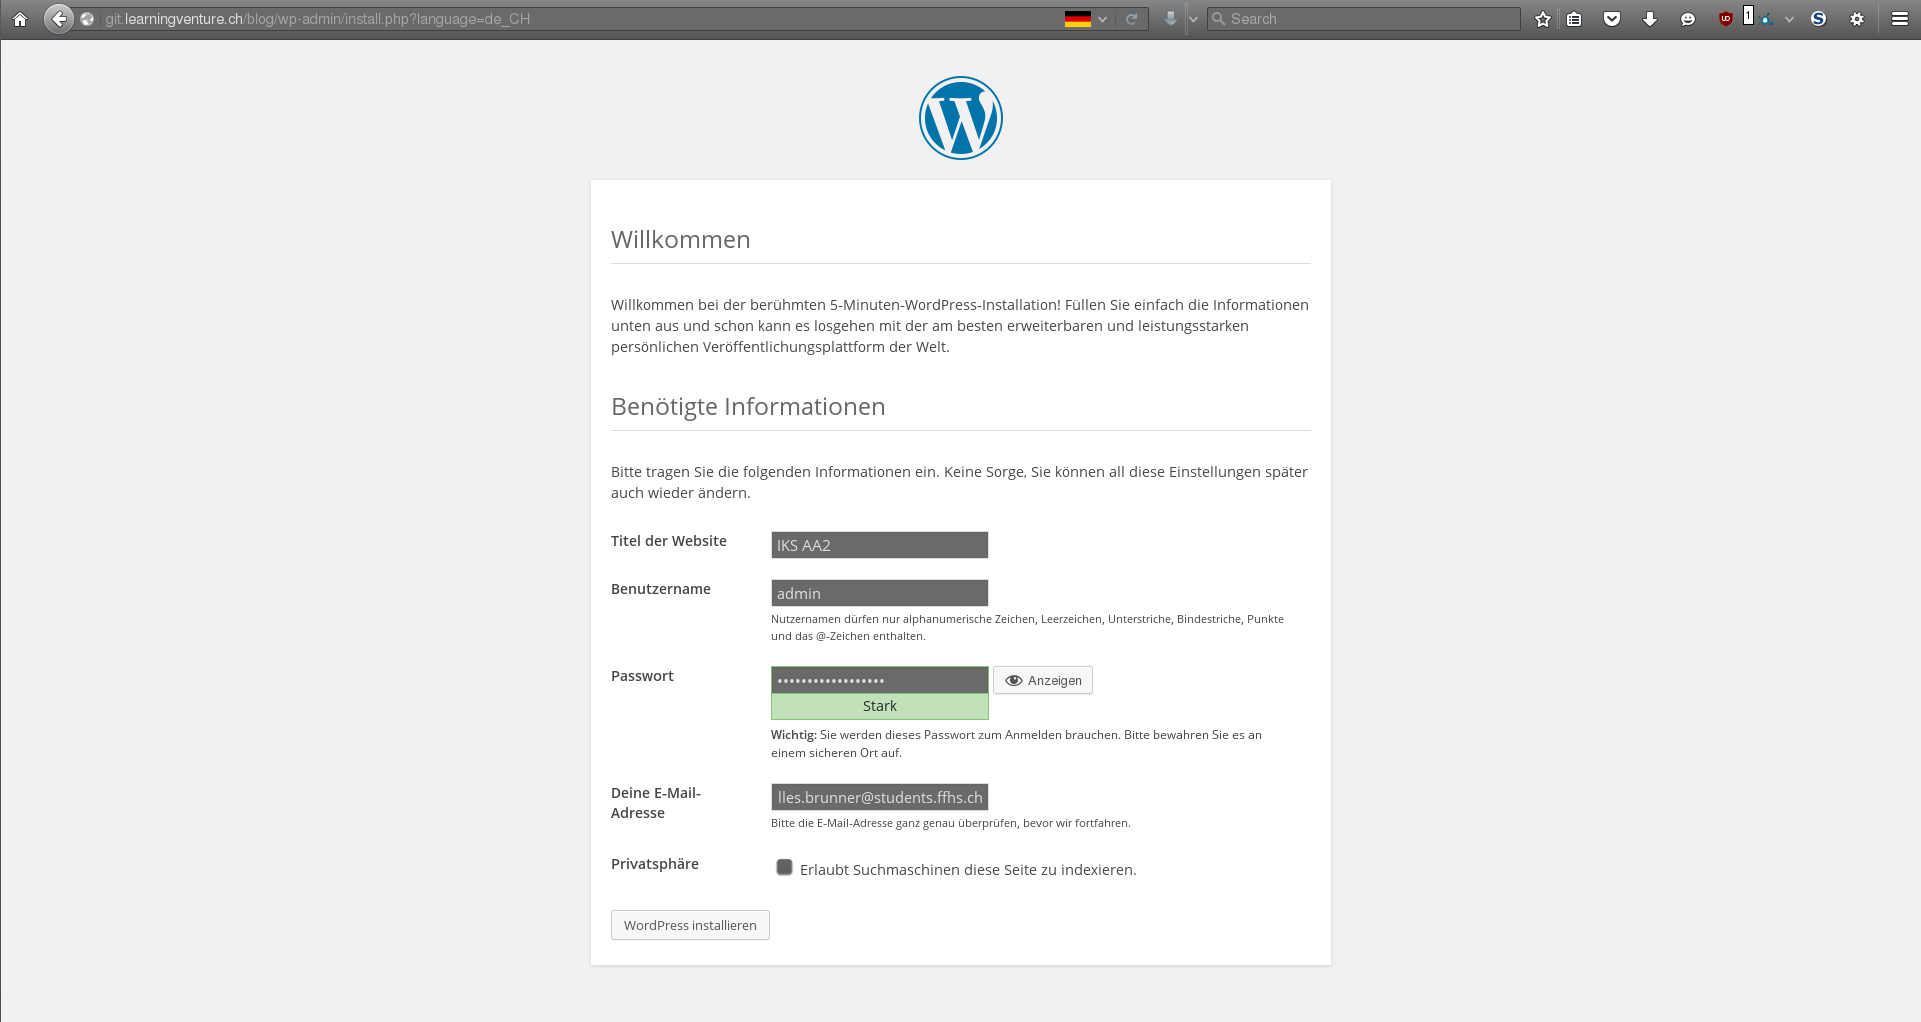
\includegraphics[width=13cm]{../Pics/38-wordpress-angaben}
	Abbildung 13: WordPress Installation
	\newline
	\newline
	Schliesslich haben wir noch wie im Arbeitsauftrag vorgegeben einen AntiSpam-Filter installiert. Abbildungen 14 und 15 illustrieren dieses Vorgehen:
	\newline
	\newline
	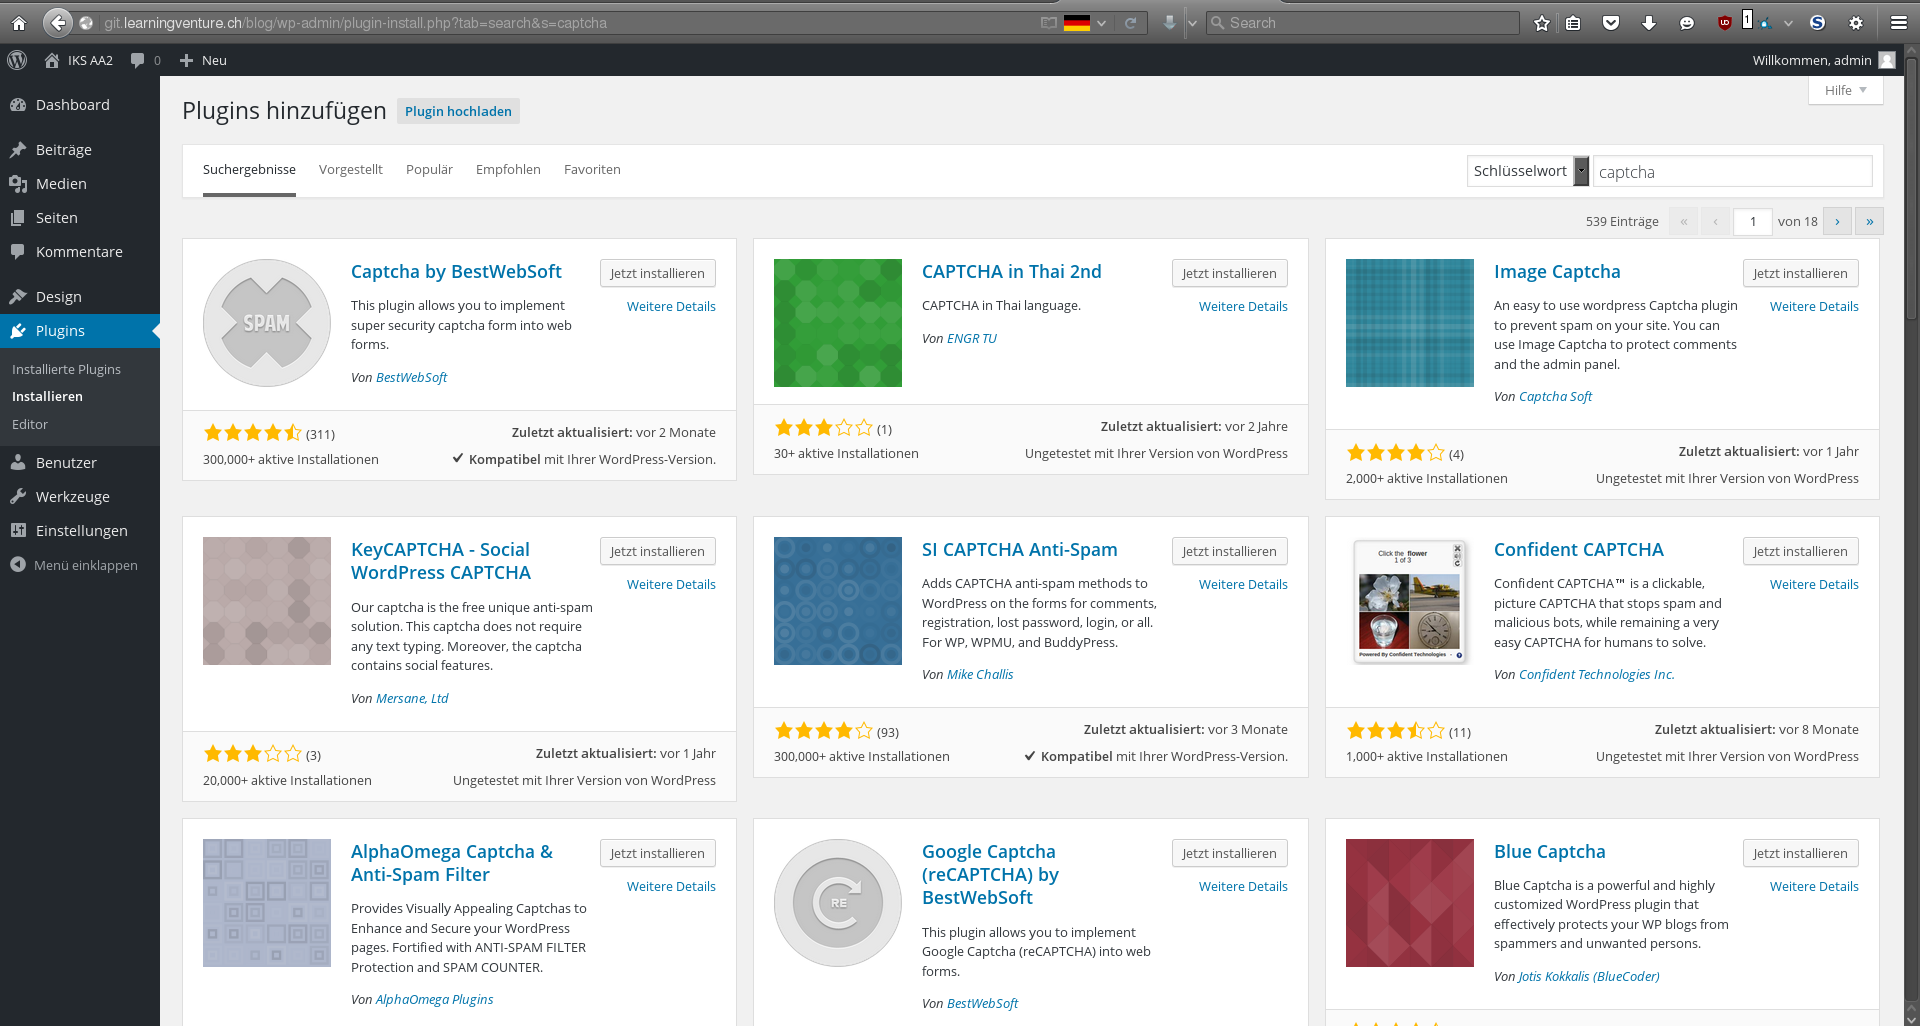
\includegraphics[width=13cm]{../Pics/40-wordpress-captcha}
	Abbildung 14: Auflistung verschiedener Captcha-Plugins
	\newline
	\newline
	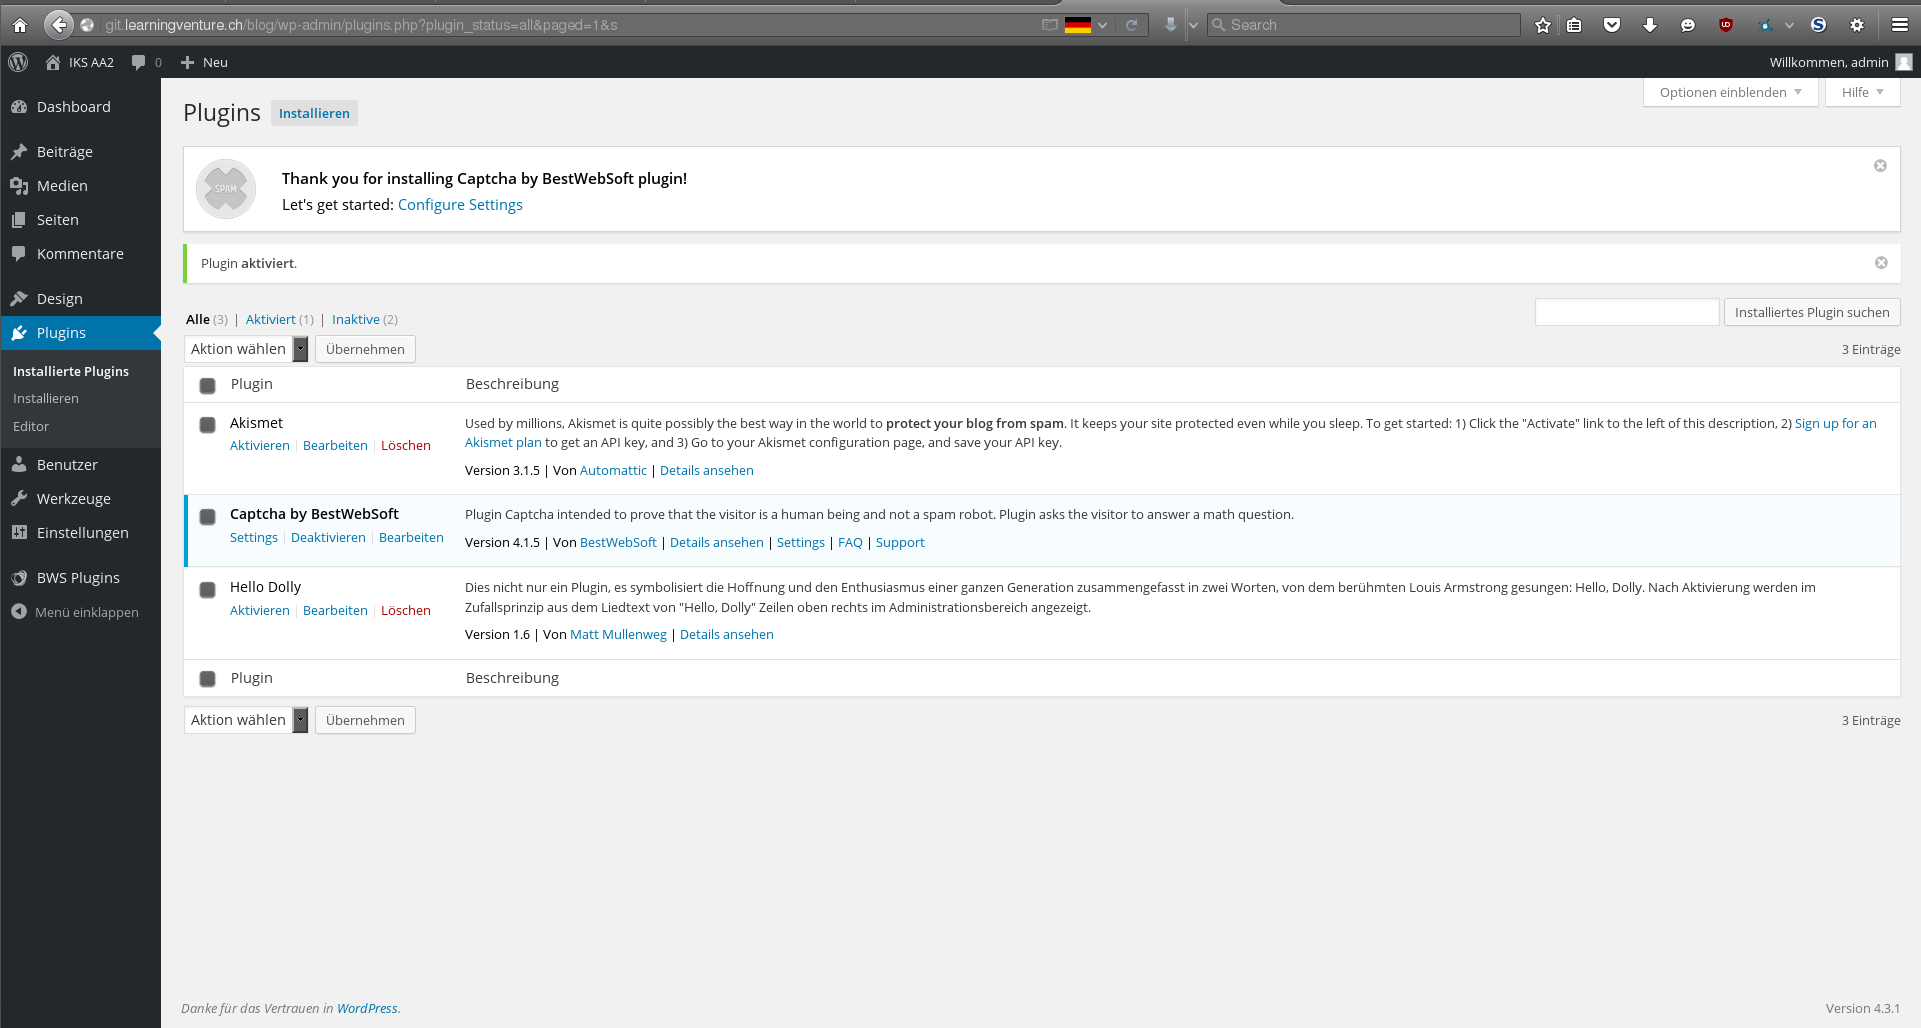
\includegraphics[width=13cm]{../Pics/41-wordpress-captcha_installed}
	Abbildung 15: Erfolgreiche Installation von Captcha by BestWebSoft
	\newline
	\newline
	\section{Schluss}
	Das oben besprochene Vorgehen führt uns Schritt für Schritt zu einer funktionierenden WordPress-Installation, die den Vorgaben unseres Arbeitsauftrags entsprechen.
	\newline
	\newline
	WordPress zu installieren ist an sich keine schwierige Aufgabe und kann innert sehr kurzer Zeit bewerkstelligt werden. Die einzige Schwierigkeit, mit der wir uns etwas länger befassen mussten, war ein korrektes Nachvollziehen und Konfigurieren der VirtualHost-Konfigurationsdatei. Nach einigen Online-Recherchen und Tests unseres Servers haben wir einen Weg gefunden, welche den Anforderungen der Aufgabe genaustens entsprechen sollte.
	\newline
	\newline
	Abschliessend sei gesagt, dass wir uns durchaus bewusst sind, dass eine laufende WordPress-Installation noch nicht bedeutet, dass unsere Arbeit getan ist. Es wird immer etwas zu konfigurieren und updaten geben. Schliesslich gilt es noch die entsprechenden Sicherheitsvorkehrungen zu treffen, da wir nicht unerwartet ungebetene Gäste auf unserem Server vorfinden oder unfreiwillig Teil eines Bot-Netzwerks werden...
\end{document}